%\RequirePackage{ifthen}
%\newboolean{longpage}
%\setboolean{longpage}{true}
%\ifthenelse{\boolean{longpage}}%
%{\documentclass[10pt]{article}}%
%{\documentclass[10pt]{book}}

\documentclass{book}

%\sffamily
\usepackage{fontspec}
%\usepackage{mathspec}
%\setallmainfonts[Mapping=tex-text]{Calibri}
%\setmainfont[Mapping=tex-text]{Calibri}
%\setsansfont[Mapping=tex-text]{Calibri}
%\setmathsfont(Greek){[cmmi10]}

%%
% slight detour to create the proper text/paper size.
% Depends on the ifthen package, needed before loading
% the geometry package
%%

\usepackage{ifthen}
\newboolean{tabletsize}
\setboolean{tabletsize}{false}


%
%	Note how the tablet version differs from the booksize only in 
% the size of the margins.
%
% Changing the following isn't hard but should be done with 
% practice and care, making sure to get the margins right for a 
% particular page size and printing format
%
%% Layout for printed book through Amazon CreateSpace, perfect bound,
%% 8.5 x 11 paper size, 1in inner margin, 1/2in (roughly) outer margin

%\usepackage{everyshi}
%\pagestyle{empty}
%\textheight500cm
%\EveryShipout{%
%\pdfpagewidth=8.5in
%\pdfpageheight=\pagetotal
%\advance\pdfpageheight by 2in
%\advance\pdfpageheight by 2\topmargin
%\advance\pdfpageheight by \textheight
%\advance\pdfpageheight by -\pagegoal}

\ifthenelse{\boolean{tabletsize}}%
						{\usepackage[paperheight=11in,paperwidth=8.5in,%
						inner=1in,includeheadfoot,textheight=9in,textwidth=345pt,%
						marginparwidth=150pt]{geometry}}%
						{\usepackage[paperheight=11in,paperwidth=8.5in,%
						inner=1in,textheight=7in,textwidth=320pt,marginparwidth=150pt,%
						marginparsep=32pt,bottom=3in,footskip=1.5in]{geometry}}
%
%\usepackage[paperheight=11in,paperwidth=8.5in, inner=1in,textheight=7in,textwidth=320pt,marginparwidth=150pt,marginparsep=32pt]{geometry}

%\setlength{\marginparwidth}{150pt}

%\textheight500cm
%\EveryShipout{%
%\pdfpagewidth=8.5in
%\pdfpageheight=\pagetotal
%\advance\pdfpageheight by 2in
%\advance\pdfpageheight by 2\topmargin
%\advance\pdfpageheight by \textheight
%\advance\pdfpageheight by -\pagegoal}



%% end detour
%%
%\newcounter{chapter}
%\newcommand{\chapter}{\refstepcounter{chapter}\Huge Chapter \thechapter \vskip 2\baselineskip\normalsize}


\usepackage{APEX_format}
%%%%
% Additional packages to support the book, not part of the APEX style.
%%%%
\usepackage{fancyhdr}
\usepackage{eso-pic}
\usepackage{lipsum}
%\usepackage{pgfplots}
%\pgfplotsset{width=\marginparwidth+1pt,compat=1.3}
\usepackage[font=small]{caption}
%,justification=centering

%%%%
%% These are low level LaTeX commands that determine the 
%% look of the Chapter and Section headings.
%% Note the use in the chapter part of an external file
%% that contains graphics for each chapter start.
%%%%

%%%%
%% Commands for the header, utilizing the fancyhdr
%% (fancy header) package
%%%%

\pagestyle{fancy}
\fancyhead{}
\fancyfoot{}
\renewcommand{\chaptermark}[1]{\markboth{\chaptername\ \thechapter\ \ \ \ {#1}}{}}
\renewcommand{\sectionmark}[1]{\markright{\thesection\ \ \ \  #1}}
\fancyhf{}         %Clears all header and footer fields, in preparation.
\renewcommand{\headrulewidth}{0pt}
\renewcommand{\footrulewidth}{0pt}

\ifthenelse{\boolean{longpage}}%
{}% end header of longpage
{% begin header/footer of not longpage
\fancyhfoffset[LE,RO]{\marginparwidth+\marginparsep}
%\fancyfoot[LE,RO]{\textbf{\thepage}} %Displays the page number in bold in the header,

\fancyfoot[LE]{\begin{minipage}{\textwidth}%
\noindent\hskip\marginparwidth\hskip\marginparsep\hskip-4pt\rule{\textwidth}{.4pt}
\vskip.2\baselineskip
\noindent\hskip\marginparwidth\hskip\marginparsep\hskip-4pt%
Notes:
\vskip 1.5in\textbf{\thepage}
\end{minipage}} 

\fancyfoot[RO]{\begin{minipage}{\textwidth+\marginparwidth+\marginparsep}%
\rule{\textwidth-\marginparwidth-\marginparsep}{.4pt}
\vskip.2\baselineskip
Notes:
\vskip 1.5in
\hfill\textbf{\thepage}
\end{minipage}}       


\fancyhead[LE]{\nouppercase{\leftmark}}
      %Displays the upper-level (chapter) information---
      % as determined above---in non-upper case in the header, 
      %to the right on even pages.
\fancyhead[RO]{\rightmark}
			%Displays the lower-level (section) information---as
      % determined above---in the header, to the left on odd pages.
      
}% End the ifthenelse{longpage}


\ifthenelse{\boolean{longpage}}% for changing the header
{% longpage
\newcommand{\exerciseheader}{}
\newcommand{\regularheader}{}
\newcommand{\endmatheader}{}
}% i.e, the above does nothing
{% now for a real change
\newcommand{\exerciseheader}{%
				\fancyhfoffset[LE,RO]{32pt}%
				\fancyfoot[LE]{\textbf{\thepage}}% 
				\fancyfoot[RO]{\textbf{\thepage}}
				\fancyhead{}% 
}

\newcommand{\regularheader}{%
\fancyhead[LE]{\nouppercase{\leftmark}}%
\fancyhead[RO]{\rightmark}%
\fancyfoot[LE]{\begin{minipage}{\textwidth}%
\noindent\hskip\marginparwidth\hskip\marginparsep\hskip-4pt\rule{\textwidth}{.4pt}
\vskip.2\baselineskip
\noindent\hskip\marginparwidth\hskip\marginparsep\hskip-4pt%
Notes:
\vskip 1.5in\textbf{\thepage}
\end{minipage}} 

\fancyfoot[RO]{\begin{minipage}{\textwidth+\marginparwidth+\marginparsep}%
\rule{\textwidth-\marginparwidth-\marginparsep}{.4pt}
\vskip.2\baselineskip
Notes:
\vskip 1.5in
\hfill\textbf{\thepage}
\end{minipage}}
\fancyhfoffset[LE,RO]{\marginparsep+\marginparwidth}
}

\newcommand{\qendheader}{%
		\fancyhead{}%
		\fancyfoot{}%
		}
}% ends if/then/else exercise/regular headers


%
%  Defining what the chapter titles look like
%

\newdimen\titleheight

\makeatletter
\def\@makechapterhead#1{%
  {\parindent \z@ \raggedright \reset@font
    {\Huge \thechapter: \scshape \textsc #1}
    \par\vskip 10\p@
    \hrule height 1pt
    \vskip 10\p@
  }}
%%  
%%%\makeatletter
%%\def\@makesectionhead#1{%
%%	 {\reset@font\LARGE\itshape\bfseries\strut #1 \thechapter.\thesection \ #1
%%	 }}

%%%%
%%
%%  For figures in the margin
%%
%%%%

%%\usepackage{wrapfig}
%%
%%\setlength{\marginparsep}{10pt}
%%\setlength{\wrapoverhang}{\marginparwidth}
%%\addtolength{\wrapoverhang}{\marginparsep}
%%
%%%\newenvironment{mfigure}[1]{%
%%%    \wrapfigure{#1}{0pt}%
%%%    \begin{minipage}{\marginparwidth}%
%%%    \centering%
%%%}{%
%%%    \end{minipage}%
%%%    \endwrapfigure%
%%%}

\counterwithin{figure}{section}

\ifthenelse{\boolean{longpage}}%
		{\newcommand{\mfigure}[5][]{%
		\vskip \baselineskip%
			\noindent\begin{minipage}{\textwidth}
  			\centering
  			\myincludegraphics{#5}
  			#1%
  			\captionsetup{type=figure}
	  		\caption{#3}\label{#4}
  		\end{minipage}
		}}
		{\newcommand{\mfigure}[5][]{%
		\ifthenelse{\isodd{\thepage}}%
			{\AddToShipoutPicture*{\put(427,\LenToUnit{#2\paperheight}){%
			\begin{minipage}{\marginparwidth}%
				\centering%
	  		\myincludegraphics[#1]{#5}%
  			\captionsetup{type=figure}%
  			%#1%
	  		\caption{#3}\label{#4}%
  		\end{minipage}}}}%
			{\AddToShipoutPicture*{\put(36,\LenToUnit{#2\paperheight}){%
			\begin{minipage}{\marginparwidth}%
			  \centering%
  		  \myincludegraphics[#1]{#5}%
  			\captionsetup{type=figure}%
  			%#1%
	  		\caption{#3}\label{#4}%
  		\end{minipage}}}}%
		}}%

\ifthenelse{\boolean{longpage}}%
		{\newcommand{\mtable}[4]{
					\vskip \baselineskip%
					\noindent\begin{minipage}{\textwidth}
  					\centering\small
  					#4
  					\captionsetup{type=figure}
	  				\caption{#2}\label{#3}
  				\end{minipage}
  				\vskip\baselineskip}
  	}
		{\newcommand{\mtable}[4]{%
			\ifthenelse{\isodd{\thepage}}%
				{\AddToShipoutPicture*{\put(427,\LenToUnit{#1\paperheight}){%
					\begin{minipage}{\marginparwidth}%
  					\centering\small%
  					#4%
  					\captionsetup{type=figure}%
	  				\caption{#2}\label{#3}%
  				\end{minipage}}}}%
				{\AddToShipoutPicture*{\put(36,\LenToUnit{#1\paperheight}){%
					\begin{minipage}{\marginparwidth}%
 						 \centering\small%
 						 #4%
						  \captionsetup{type=figure}%
	  					\caption{#2}\label{#3}%
 					 \end{minipage}}}}%
		}}%

\ifthenelse{\boolean{longpage}}%
		{\newcommand{\mnote}[2]{%
					\hskip 25pt%
					\begin{minipage}{250pt}%
					\small%
					#2%
					\end{minipage}%
					\vskip\baselineskip%
		}%
		}%
		{\newcommand{\mnote}[2]{%
			\ifthenelse{\isodd{\thepage}}%
				{\AddToShipoutPicture*{\put(427,\LenToUnit{#1\paperheight}){%
					\begin{minipage}{\marginparwidth}
  					\small
  					#2
  				\end{minipage}}}}%
				{\AddToShipoutPicture*{\put(36,\LenToUnit{#1\paperheight}){%
					\begin{minipage}{\marginparwidth}
 						 \small
 						 #2
					\end{minipage}}}}
		}}


\newcommand{\showheightguidelines}{%
\AddToShipoutPicture{\put(10,\LenToUnit{.1\paperheight}){\tiny 10\%\rule{10pt}{1pt}}}
\AddToShipoutPicture{\put(10,\LenToUnit{.2\paperheight}){\tiny 20\%\rule{10pt}{1pt}}}
\AddToShipoutPicture{\put(10,\LenToUnit{.3\paperheight}){\tiny 30\%\rule{10pt}{1pt}}}
\AddToShipoutPicture{\put(10,\LenToUnit{.4\paperheight}){\tiny 40\%\rule{10pt}{1pt}}}
\AddToShipoutPicture{\put(10,\LenToUnit{.5\paperheight}){\tiny 50\%\rule{10pt}{1pt}}}
\AddToShipoutPicture{\put(10,\LenToUnit{.6\paperheight}){\tiny 60\%\rule{10pt}{1pt}}}
\AddToShipoutPicture{\put(10,\LenToUnit{.7\paperheight}){\tiny 70\%\rule{10pt}{1pt}}}
\AddToShipoutPicture{\put(10,\LenToUnit{.8\paperheight}){\tiny 80\%\rule{10pt}{1pt}}}
\AddToShipoutPicture{\put(10,\LenToUnit{.9\paperheight}){\tiny 90\%\rule{10pt}{1pt}}}
\AddToShipoutPicture{\put(580,\LenToUnit{.1\paperheight}){\rule{10pt}{1pt}\tiny 10\%}}
\AddToShipoutPicture{\put(580,\LenToUnit{.2\paperheight}){\rule{10pt}{1pt}\tiny 20\%}}
\AddToShipoutPicture{\put(580,\LenToUnit{.3\paperheight}){\rule{10pt}{1pt}\tiny 30\%}}
\AddToShipoutPicture{\put(580,\LenToUnit{.4\paperheight}){\rule{10pt}{1pt}\tiny 40\%}}
\AddToShipoutPicture{\put(580,\LenToUnit{.5\paperheight}){\rule{10pt}{1pt}\tiny 50\%}}
\AddToShipoutPicture{\put(580,\LenToUnit{.6\paperheight}){\rule{10pt}{1pt}\tiny 60\%}}
\AddToShipoutPicture{\put(580,\LenToUnit{.7\paperheight}){\rule{10pt}{1pt}\tiny 70\%}}
\AddToShipoutPicture{\put(580,\LenToUnit{.8\paperheight}){\rule{10pt}{1pt}\tiny 80\%}}
\AddToShipoutPicture{\put(580,\LenToUnit{.9\paperheight}){\rule{10pt}{1pt}\tiny 90\%}}
}

%\ifthenelse{\boolean{longpage}}%
		%{}
		%{\newcommand{\mfigurethree}[5][]{%
		%\ifthenelse{\isodd{\thepage}}%
			%{\AddToShipoutPicture*{\put(427,\LenToUnit{#2\paperheight}){%
			%\begin{minipage}{\marginparwidth}%
				%\centering%
	  		%\includemedia[#1]{\includegraphics{#5}}{#5.prc}%
  			%\captionsetup{type=figure}%
  			%%#1%
	  		%\caption{#3}\label{#4}%
  		%\end{minipage}}}}%
			%{\AddToShipoutPicture*{\put(36,\LenToUnit{#2\paperheight}){%
			%\begin{minipage}{\marginparwidth}%
			  %\centering%
  			%\includemedia[#1]{\includegraphics{#5}}{#5.prc}%
  			%\captionsetup{type=figure}%
  			%%#1%
	  		%\caption{#3}\label{#4}%
  		%\end{minipage}}}}%
		%}}%
		
		\newcommand{\mfigurethree}[6]{%
		\ifthenelse{\isodd{\thepage}}%
			{\AddToShipoutPicture*{\put(427,\LenToUnit{#3\paperheight}){%
			\begin{minipage}{\marginparwidth}%
				\centering%
				\ifthenelse{\boolean{in_threeD}}{% in 3D
	  		\includemedia[#1]{\includegraphics[#2]{#6_3D\colornamesuffix}}{#6_3D.prc}}%now not in 3D
				{\myincludegraphics[#2]{#6}}%
  			\captionsetup{type=figure}%
  			%#1%
	  		\caption{#4}\label{#5}%
  		\end{minipage}}}}%
			{\AddToShipoutPicture*{\put(36,\LenToUnit{#3\paperheight}){%
			\begin{minipage}{\marginparwidth}%
			  \centering%
  			\ifthenelse{\boolean{in_threeD}}{% in 3D
	  		\includemedia[#1]{\includegraphics[#2]{#6_3D\colornamesuffix}}{#6_3D.prc}}%now not in 3D
				{\myincludegraphics[#2]{#6}}%
  			\captionsetup{type=figure}%
  			%#1%
	  		\caption{#4}\label{#5}%
  		\end{minipage}}}}%
		}

%\AddToShipoutPicture{\ifthenelse{\ifodd{\thepage}}%
%{\put(10,10){\begin{tikzpicture}\draw (0,0) circle (5pt);\end{tikzpicture}}}%
%{\put(100,100){\begin{tikzpicture}\draw (0,0) circle (5pt);\end{tikzpicture}}}}%
%

%\AddToShipoutPictureBG{%
% \AtPageLowerLeft{\hspace{1cm}A small logo: \rule{2cm}{3cm}}}
% 
%}{\AddToShipoutPicture*{\put(36,\LenToUnit{#2\paperheight})}}%
%{%
%\begin{minipage}{\marginparwidth}
%  \centering
%  \includegraphics{#1}
%  \captionof{figure}{#3}
%  \end{minipage}}}
%\AddToShipoutPicture*{\put(\LenToUnit{.5\paperwidth},\LenToUnit{.75\paperheight}){%
%  \begin{minipage}{100pt}
%  \centering
%  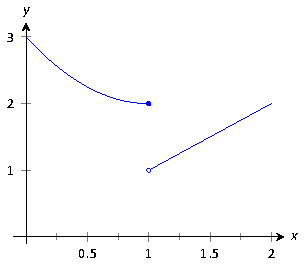
\includegraphics{test-figure2.pdf}
%  \captionof{figure}{Test caption}
%  \end{minipage}}}


%\newenvironment{mfigurefile}[2]{%
%\begin{tikzpicture}[remember picture,overlay]%
%\ifthenelse{\isodd{\thepage}}{\node [xshift=-36pt-.5\marginparwidth,yshift=#2\paperheight] at (current page.south east) }{\node [xshift=36pt+.5\marginparwidth,yshift=#2\paperheight] at (current page.south west) }%
%{\input{#1}};}%
%{\end{tikzpicture}%
%}

%\DeclareCaptionType{mytype}[Typename][List of mytype]


    
%%%%
%% End margin figure 
%%%%    
    

\newcommand{\bmx}[1]{\left[\hskip -3pt\begin{array}{#1} }
\newcommand{\emx}{\end{array}\hskip -3pt\right]}

\newcommand{\btz}{\begin{center}\begin{tikzpicture}}
\newcommand{\etz}{\end{tikzpicture}\end{center}}

\newcommand{\ds}{\displaystyle}

\newcommand{\fp}{\ensuremath{f\,'}}
\newcommand{\fpp}{\ensuremath{f\,''}}

\newcommand{\Fp}{\ensuremath{F\primeskip'}}
\newcommand{\Fpp}{\ensuremath{F\primeskip''}}

\newcommand{\yp}{\ensuremath{y\primeskip'}}
\newcommand{\gp}{\ensuremath{g\primeskip'}}

\newcommand{\dx}{\ensuremath{\Delta x}}
\newcommand{\dy}{\ensuremath{\Delta y}}
%\newcommand{\dz}{\ensuremath{\Delta z}}
\newcommand{\ddz}{\ensuremath{\Delta z}}

\newcommand{\thet}{\ensuremath{\theta}}
\newcommand{\norm}[1]{\ensuremath{||\ #1\ ||}}
\newcommand{\vnorm}[1]{\ensuremath{\norm{\vec #1}}}
\newcommand{\snorm}[1]{\ensuremath{\left|\left|\ #1\ \right|\right|}}
\newcommand{\la}{\left\langle}
\newcommand{\ra}{\right\rangle}
\newcommand{\dotp}[2]{\ensuremath{\vec #1 \cdot \vec #2}}
\newcommand{\proj}[2]{\ensuremath{\text{proj}_{\,\vec #2}{\,\vec #1}}}
\newcommand{\crossp}[2]{\ensuremath{\vec #1 \times \vec #2}}
\newcommand{\veci}{\ensuremath{\vec i}}
\newcommand{\vecj}{\ensuremath{\vec j}}
\newcommand{\veck}{\ensuremath{\vec k}}
\newcommand{\vecu}{\ensuremath{\vec u}}
\newcommand{\vecv}{\ensuremath{\vec v}}
\newcommand{\vecw}{\ensuremath{\vec w}}
\newcommand{\vecx}{\ensuremath{\vec x}}
\newcommand{\vecy}{\ensuremath{\vec y}}
\newcommand{\vrp}{\ensuremath{\vec r\, '}}
\newcommand{\vsp}{\ensuremath{\vec s\, '}}
\newcommand{\vrt}{\ensuremath{\vec r(t)}}
\newcommand{\vst}{\ensuremath{\vec s(t)}}
\newcommand{\vvt}{\ensuremath{\vec v(t)}}
\newcommand{\vat}{\ensuremath{\vec a(t)}}
\newcommand{\px}{\ensuremath{\partial x}}
\newcommand{\py}{\ensuremath{\partial y}}
\newcommand{\pz}{\ensuremath{\partial z}}
\newcommand{\pf}{\ensuremath{\partial f}}
\newcommand{\underlinespace}{\underline{\phantom{xxxxxx}}}

\newcommand{\surfaceS}{\ensuremath{\mathcal{S}}}

\newcommand{\mathN}{\ensuremath{\mathbb{N}}}

\newcommand{\zerooverzero}{\ensuremath{\ds \raisebox{8pt}{\text{``\ }}\frac{0}{0}\raisebox{8pt}{\text{\ ''}}}}


\newcommand{\myrule}{\rule[-4pt]{0pt}{13pt}}
\newcommand{\mmrule}{\rule[-10pt]{0pt}{15pt}}
\newcommand{\myds}{\ds\mmrule}
\newcommand{\deriv}[2]{\ensuremath{\myds\frac{d}{dx}\left(#1\right)=#2}}
\newcommand{\myint}[2]{\ensuremath{\myds\int #1\ dx=} \ensuremath{\ds #2}}

\DeclareMathOperator{\sech}{sech}
\DeclareMathOperator{\csch}{csch}
\DeclareMathOperator{\curl}{curl}
\DeclareMathOperator{\divv}{div}

\newcommand{\sword}[1]{\textbf{#1}}

\newcommand{\primeskip}{\hskip.75pt}

%%%% Begin Header TikZ

%  Some TiKZ  shortcuts to help make drawing 3D vectors faster.
%

\newcommand{\plotlinecolor}{blue}

%
% Draw x and y tick marks
%
\newcommand{\drawxticks}[1]
{\foreach \x in {#1}
		{\draw  (\x,-.1)--(\x,.1);
			};
}
\newcommand{\drawyticks}[1]
{\foreach \x in {#1}
		{\draw  (-.1,\x)--(.1,\x);
			};
}

\newcommand{\drawxlines}[3]
{\draw[<->] (#1,0) -- (#2,0) node [right] {$x$};
\foreach \x in {#3}
		{\draw  (\x,-.1)--(\x,.1);
			};
}

\newcommand{\drawylines}[3]
{\draw[<->] (0,#1) -- (0,#2) node [above] {$y$};
\foreach \x in {#3}
		{\draw  (-.1,\x)--(.1,\x);
			};
}

\newcommand{\drawxlabels}[1]
{\foreach \x in {#1}
		{\draw  (\x,-.1) node [below] {\scriptsize $\x$};
		};
}

\newcommand{\drawylabels}[1]
{\foreach \x in {#1}
		{\draw  (-.1,\x) node [left] {\scriptsize $\x$};
		};
}

%% draw a box of margin width size to see if figure is properly contained within
\newcommand{\marginsizebox}{\draw (0,0)--(\marginparwidth,0)--(\marginparwidth,3)--(0,3)--cycle;}

%%%%
%%%%

\newcommand{\asyouread}[1]{\begin{tikzpicture}
\ifthenelse{\boolean{in_color}}{\node [preaction={fill=black,opacity=.5,transform canvas={xshift=1mm,yshift=-1mm}}, right color=blue!80!black!30, left color=blue!80] at (0,0) {\textcolor{white}{\textsf{\textit{AS YOU READ $\ldots$}}}};}
{\node [preaction={fill=black,opacity=.5,transform canvas={xshift=1mm,yshift=-1mm}}, right color=black!30, left color=black!10] at (0,0) {\textcolor{white}{\textsf{\textit{AS YOU READ $\ldots$}}}};}
\end{tikzpicture}
\begin{enumerate}
#1
\end{enumerate}
\vskip 20pt}

%%%%
%%  A new figure environment, trying to fix the float problem.
%%
%%%%

%\newcounter{myfigurecounter}[chapter]
%\renewcommand\themyfigurecounter{\thechapter.\arabic{myfigurecounter}}
%\newenvironment{myfigure}{\refstepcounter{myfigurecounter}}{}
%\newcommand{\mycaption}[1]{%
%\begin{center}%
%\vskip -1.5\baselineskip
%\begin{tikzpicture}%
%\draw (0,0) node [text width=\textwidth,align=center] {Figure \themyfigurecounter: #1};%
%\end{tikzpicture}%
%\end{center}%
%}

%\pgfrealjobname{Calculus}



\begin{document}

%%%%%%%%%%
%%%
%%%  Set criteria for the format of the book.
%%%  This supercedes anything set in the Text_Header.
%%%
%%%%%%%%%%


\printincolor
%\printinblackandwhite

%\printexercisenames

%\nodrawexamplelines

%\printallanswers


\normalem


\chapter{Limits}\label{chapter:limits}
%\thispagestyle{empty}

\textit{Calculus} means ``a method of calculation or reasoning.'' When one computes the sales tax on a purchase, one employs a simple calculus. When one finds the area of a polygonal shape by breaking it up into a set of triangles, one is using another calculus. Proving a theorem in geometry employs yet another calculus.

Despite the wonderful advances in mathematics that had taken place into the first half of the $17^\text{th}$ century, mathematicians and scientists were keenly aware of what they \textit{could not do.} (This is true even today.) In particular, two important concepts eluded mastery by the great thinkers of that time: area and rates of change. 

Area seems innocuous enough; areas of circles, rectangles, parallelograms, etc., are standard topics of study for students today just as they were then. However, the areas of \textit{arbitrary} shapes could not be computed, even if the boundary of the shape could be described exactly. 

Rates of change were also important. When an object moves at a constant rate of change, then ``distance = rate $\times $ time.'' But what if the rate is not constant -- can distance still be computed? Or, if distance is known, can we discover the rate of change?

It turns out that these two concepts were related. Two mathematicians, Sir Isaac Newton and Gottfried Leibniz, are credited with independently formulating a system of computing that solved the above problems and showed how they were connected. Their system of reasoning was ``a'' calculus. However, as the power and importance of their discovery took hold, it became known to many as ``the'' calculus. Today, we generally shorten this to discuss ``calculus.''

The foundation of ``the calculus'' is the \textit{limit.} It is a tool to describe a particular behavior of a function. This chapter begins our study of the limit by approximating its value graphically and numerically. After a formal definition of the limit, properties are established that make ``finding limits'' tractable. Once the limit is understood, then the problems of area and rates of change can be approached.



\section{An Introduction To Limits}\label{sec:limit_intro}

We begin our study of \textit{limits} by considering examples that demonstrate key concepts that will be explained as we progress.\\

Consider the function $y = \frac{\sin x}{x}$. When $x$ is near the value 1, what value (if any) is $y$ near?%

While our question is not precisely formed (what constitutes ``near the value 1''?), the answer does not seem difficult to find. One might think first to look at a graph of this function to approximate the appropriate $y$ values. Consider Figure \ref{fig:zoom_sinx_over_x}, where $y = \frac{\sin x}{x}$ is graphed. For values of $x$ near 1, it seems that $y$ takes on values near $0.85$. In fact, when $x=1$, then $y=\frac{\sin 1}{1} \approx 0.84$, so it makes sense that when $x$ is ``near'' 1, $y$ will be ``near'' $0.84$.

\mfigure{.8}{$\sin(x)/x$ near $x=1$.}{fig:zoom_sinx_over_x}{figures/figZoomSinXOverX}
\mfigure{.55}{$\sin(x)/x$ near $x=0$.}{fig:sinx_over_x}{figures/figSinXOverX}
Consider this again at a different value for $x$. When $x$ is near 0, what value (if any) is $y$ near? By considering Figure \ref{fig:sinx_over_x}, one can see that it seems that $y$ takes on values near $1$. But what happens when $x=0$? We have $$ y \rightarrow \frac{\sin 0}{0} \rightarrow \raisebox{8pt}{\text{``\ }}\frac{0}{0}\raisebox{8pt}{\text{\ ''}}.$$ 
The expression ``$0/0$'' has no value; it is \emph{indeterminate.} \index{limit!indeterminate form}\index{indeterminate form} Such an expression gives no information about what is going on with the function nearby. We cannot find out how $y$ behaves near $x=0$ for this function simply by letting $x=0$. 

\emph{Finding a limit} entails understanding how a function behaves near a particular value of $x$. Before continuing, it will be useful to establish some notation. Let $y=f(x)$; that is, let $y$ be a function of $x$ for some function $f$. The expression ``the limit of $y$ as $x$ approaches 1'' describes a number, often referred to as $L$, that $y$ nears as $x$ nears 1. We write all this as $$\lim_{x\to 1} y = \lim_{x\to 1} f(x) = L.$$ This is not a complete definition (that will come in the next section); this is a pseudo-definition that will allow us to explore the idea of a limit. \index{limit!pseudo-definition}

Above, where $f(x) = \sin(x)/x$, we approximated $$\lim_{x\to 1} \frac{\sin x}{x} \approx 0.84 \quad \text{ and } \quad \lim_{x\to 0}\frac{\sin x}{x} \approx 1.$$ (We \textit{approximated} these limits, hence used the ``$\approx$'' symbol, since we are working with the pseudo-definition of a limit, not the actual definition.)

Once we have the true definition of a limit, we will find limits \textit{analytically}; that is, exactly using a variety of mathematical tools. For now, we will \textit{approximate} limits both graphically and numerically. Graphing a function can provide a good approximation, though often not very precise. Numerical methods can provide a more accurate approximation. We have already approximated limits graphically, so we now turn our attention to numerical approximations.


Consider again $\lim_{x\to 1}\sin (x)/x$. To approximate this limit numerically, we can create a table of $x$ and $f(x)$ values where $x$ is ``near'' 1. This is done in Figure \ref{table:sinx_1}.\par

Notice that for values of $x$ near $1$, we have $\sin (x)/x$ near $0.841$. The $x=1$ row is in bold to highlight the fact that when considering limits, we are \textit{not} concerned with the value of the function at that particular $x$ value; we are only concerned with the values of the function when $x$ is \textit{near} 1. 

\mtable{.3}{Values of $\sin(x)/x$ with $x$ near 1.}{table:sinx_1}{\begin{tabular}{cc}
$x$ & $\sin(x)/x$ \\ \hline 
0.9 & 0.870363 \\
 0.99 & 0.844471 \\
 0.999 & 0.841772 \\
 \textbf{1} & \textbf{0.841471} \\
 1.001 & 0.84117 \\
 1.01 & 0.838447 \\
 1.1 & 0.810189
\end{tabular}
%\caption{Values of $\frac{\sin x}{x}$ for $x$ near 1.}\label{fig:sinx_1_table}
}

%\vskip \baselineskip

Now approximate $\lim_{x\to 0} \sin(x)/x$ numerically. We already approximated the value of this limit as 1 graphically in Figure \ref{fig:sinx_over_x}. The table in Figure \ref{table:sinx_2} shows the value of $\sin(x)/x$ for values of $x$ near 0. Ten places after the decimal point are shown to highlight how close to 1 the value of $\sin(x)/x$ gets as $x$ takes on values very near 0. We include the $x=0$ row in bold again to stress that we are not concerned with the value of our function at $x=0$, only on the behavior of the function \textit{near} 0. 

\mtable{.8}{Values of $\sin(x)/x$ with $x$ near 0.}{table:sinx_2}{\begin{tabular}{cc}
$x$ & $\sin(x)/x$ \\ \hline
 -0.1 & 0.9983341665 \\
 -0.01 & 0.9999833334 \\
 -0.001 & 0.9999998333 \\
 \textbf{0} & \textbf{not defined} \\
 0.001 & 0.9999998333 \\
 0.01 & 0.9999833334 \\
 0.1 & 0.9983341665
 \end{tabular}
% \caption{Values of $\frac{\sin x}{x}$ for $x$ near 0.}\label{fig:sinx_0_table}}
 
This numerical method gives confidence to say that 1 is a good approximation of $\lim_{x\to 0} \sin(x)/x$; that is, $$\lim_{x\to 0} \sin(x)/x \approx 1.$$ Later we will be able to prove that the limit is \textit{exactly} 1.

We now consider several examples that allow us explore different aspects of the limit concept.\\

\mfigure{.55}{Graphically approximating a limit in Example \ref{ex_limit1}.}{fig:limit1}{figures/figlimit1}
\mtable{.35}{Numerically approximating a limit in Example \ref{ex_limit1}.}{table:limit1}{\begin{tabular}{cc}
$x$ & $\frac{x^2-x-6}{6x^2-19x+3}$ \\ \hline
2.9 & 0.29878 \\
 2.99 & 0.294569 \\
 2.999 & 0.294163 \\
 \textbf{3} & \textbf{not defined}\\
 3.001 & 0.294073 \\
 3.01 & 0.293669 \\
 3.1 & 0.289773
 \end{tabular}
}

\example{ex_limit1}{Approximating the value of a limit}{
Use graphical and numerical methods to approximate $$\lim_{x\to 3} \frac{x^2-x-6}{6x^2-19x+3}.$$}%
{To graphically approximate the limit, graph $$y = (x^2-x-6)/(6x^2-19x+3)$$ on a small interval that contains 3. To numerically approximate the limit, create a table of values where the $x$ values are near 3. This is done in Figures \ref{fig:limit1} and \ref{table:limit1}, respectively.

\enlargethispage{2\baselineskip}

The graph shows that when $x$ is near 3, the value of $y$ is very near $0.3$. By considering values of $x$ near 3, we see that $y=0.294$ is a better approximation. The graph and the table imply that $$\lim_{x\to 3} \frac{x^2-x-6}{6x^2-19x+3} \approx 0.294.$$ 
\vskip -\baselineskip
}\\

This example may bring up a few questions about approximating limits (and the nature of limits themselves). 
\begin{enumerate}
\item		If a graph does not produce as good an approximation as a table, why bother with it?
\item		How many values of $x$ in a table are ``enough?'' In the previous example, could we have just used $x=3.001$ and found a fine approximation?
\end{enumerate}

Graphs are useful since they give a visual understanding concerning the behavior of a function. Sometimes a function may act ``erratically'' near certain $x$ values which is hard to discern numerically but very plain graphically. Since graphing utilities are very accessible, it makes sense to make proper use of them.


Since tables and graphs are used only to \textit{approximate} the value of a limit, there is not a firm answer to how many data points are ``enough.'' Include enough so that a trend is clear, and use values (when possible) both less than and greater than the value in question. In Example \ref{ex_limit1}, we used both values less than and greater than 3. Had we used just $x=3.001$, we might have been tempted to conclude that the limit had a value of $0.3$. While this is not far off, we could do better. Using values ``on both sides of 3'' helps us identify trends.\\

\example{ex_limit2}{Approximating the value of a limit}{
Graphically and numerically approximate the limit of $f(x)$ as $x$ approaches 0, where $$f(x) = \left\{\begin{array}{rl} x+1 & x< 0 \\ -x^2+1 & x > 0 \end{array}\right..$$}{Again we graph $f(x)$ and create a table of its values near $x=0$ to approximate the limit. Note that this is a piecewise defined function, so it behaves differently on either side of 0. Figure \ref{fig:limit2} shows a graph of $f(x)$, and on either side of 0 it seems the $y$ values approach 1. Note that $f(0)$ is not actually defined, as indicated in the graph with the open circle.

\mfigure{.65}{Graphically approximating a limit in Example \ref{ex_limit2}.}{fig:limit2}{figures/figlimit2}
\mtable{.45}{Numerically approximating a limit in Example \ref{ex_limit2}.}{table:limit2}{\begin{tabular}{cc}
$x$ & $f(x)$ \\ \hline
-0.1 & 0.9 \\
 -0.01 & 0.99 \\
 -0.001 & 0.999 \\
 0.001 & 0.999999 \\
 0.01 & 0.9999 \\
 0.1 & 0.99
 \end{tabular}
}

The table shown in Figure \ref{table:limit2} shows values of $f(x)$ for values of $x$ near 0. It is clear that as $x$ takes on values very near 0, $f(x)$ takes on values very near 1. It turns out that if we let $x=0$ for either ``piece'' of $f(x)$, 1 is returned; this is significant and we'll return to this idea later.

The graph and table allow us to say that $\lim_{x\to 0}f(x) \approx 1$; in fact, we are probably very sure it \emph{equals} 1.
}\\

\enlargethispage{\baselineskip}
\vskip \baselineskip
\noindent\textbf{\large Identifying When Limits Do Not Exist}\\

A function may not have a limit for all values of $x$. That is, we cannot say $\lim_{x\to c}f(x)=L$ for some numbers $L$ for all values of $c$, for there may not be a number that $f(x)$ is approaching. There are three common ways in which a limit may fail to exist. \index{limit!does not exist}
\begin{enumerate}
\item		The function $f(x)$ may approach different values on either side of $c$.
\item		The function may grow without upper or lower bound as $x$ approaches $c$.
\item		The function may oscillate as $x$ approaches $c$ without approaching a specific value.
\end{enumerate}

We'll explore each of these in turn.\\

\vskip \baselineskip

%\noindent
%

\example{ex_no_limit1}{Different Values Approached From Left and Right}{
Explore why $\ds\lim_{x\to 1} f(x)$ does not exist, where $$f(x) = \left\{\begin{array}{cl} x^2-2x+3 & x\leq 1 \\ x & x>1 \end{array}\right..$$}%
{
A graph of $f(x)$ around $x=1$ and a table are given in Figures \ref{fig:nolimit1} and \ref{table:nolimit1}, respectively. It is clear that as $x$ approaches 1, $f(x)$ does not seem to approach a single number. Instead, it seems as though $f(x)$ approaches two different numbers. When considering values of $x$ less than 1 (approaching 1 from the left), it seems that $f(x)$ is approaching 2; when considering values of $x$ greater than 1 (approaching 1 from the right), it seems that $f(x)$ is approaching 1. Recognizing this behavior is important; we'll study this in greater depth later. Right now, it suffices to say that the limit does not exist since $f(x)$ is not approaching one value as $x$ approaches 1.
\mfigure{.8}{Observing no limit as $x\to 1$ in Example \ref{ex_no_limit1}.}{fig:nolimit1}{figures/fignolimit1}
\mtable{.6}{Values of $f(x)$ near $x=1$ in Example \ref{ex_no_limit1}.}{table:nolimit1}{\begin{tabular}{cc}
$x$ & $f(x)$ \\ \hline
 0.9 & 2.01 \\
 0.99 & 2.0001 \\
 0.999 & 2.000001 \\
 1.001 & 1.001 \\
 1.01 & 1.01 \\
 1.1 & 1.1
\end{tabular}
}
}\\

%
%\vskip \baselineskip
%\noindent\textbf{The Function Grows Without Bound}\\

%\begin{tikzpicture}
\begin{axis}[width=\marginparwidth+25pt,tick label style={font=\scriptsize},minor x tick num=1,axis y line=middle,axis x line=middle,ymin=-1,ymax=110,xmin=-.1,xmax=2.1,name=myplot]

\addplot [{\colorone},smooth,thick] coordinates {(0.,1.) (0.05,1.10803) (0.1,1.23457) (0.15,1.38408) (0.2,1.5625)(0.25,1.77778) (0.3,2.04082) (0.35,2.36686) (0.4,2.77778)(0.45,3.30579) (0.5,4.) (0.55,4.93827) (0.6,6.25) (0.65,8.16327)(0.7,11.1111) (0.75,16.) (0.8,25.) (0.85,44.4444) (0.9,100.) };
\addplot [{\colorone},smooth,thick] coordinates {(1.1,100.) (1.15,44.4444) (1.2,25.) (1.25,16.) (1.3,11.1111) (1.35,8.16327) (1.4,6.25) (1.45,4.93827) (1.5,4.) (1.55,3.30579) (1.6,2.77778) (1.65,2.36686) (1.7,2.04082) (1.75,1.77778) (1.8,1.5625) (1.85,1.38408) (1.9,1.23457) (1.95,1.10803) (2.,1.)};
%\addplot [{\colorone},smooth] coordinates {(1,1) (1.1,1.1) (1.2,1.2) (1.3,1.3) (1.4,1.4) (1.5,1.5) (1.6,1.6) (1.7,1.7) (1.8,1.8) (1.9,1.9) (2.,2.)
\draw [dashed,thick] (axis cs: 1,1) -- (axis cs: 1,100);
\end{axis}
\node [right] at (myplot.right of origin) {\scriptsize $x$};
\node [above] at (myplot.above origin) {\scriptsize $y$};
\end{tikzpicture}
%\caption{of $f(x)$ in Example \ref{ex_no_limit2}.}\label{fig:nolimit2}
\example{ex_no_limit2}{The Function Grows Without Bound}{
Explore why $\ds\lim_{x\to 1} 1/(x-1)^2$ does not exist.}%
{A graph and table of $f(x) = 1/(x-1)^2$ are given in Figures \ref{fig:nolimit2} and \ref{table:nolimit2}, respectively. Both show that as $x$ approaches 1, $f(x)$ grows larger and larger. 
\mfigure{.4}{Observing no limit as $x\to 1$ in Example \ref{ex_no_limit2}.}{fig:nolimit2}{figures/fignolimit2}
\mtable{.2}{Values of $f(x)$ near $x=1$ in Example \ref{ex_no_limit2}.}{table:nolimit2}{\begin{tabular}{cc}
$x$ & $f(x)$ \\ \hline
 0.9 & 100. \\
 0.99 & 10000. \\
 0.999 & $1.\times 10^6$ \\
 1.001 & $1.\times 10^6$ \\
 1.01 & 10000. \\
 1.1 & 100.
\end{tabular}}

We can deduce this on our own, without the aid of the graph and table. If $x$ is near 1, then $(x-1)^2$ is very small, and: $$\frac{1}{\text{very small number}} = \text{very large number}.$$
Since $f(x)$ is not approaching a single number, we conclude that $$\lim_{x\to 1}\frac{1}{(x-1)^2}$$ does not exist.
}\\

%\vskip \baselineskip
%\noindent\textbf{The Function Oscillates}\\

\example{ex_no_limit3}{The Function Oscillates}{
Explore why $\ds\lim_{x\to 0}\sin(1/x)$ does not exist.}%
{%\mfigure{.4}{Observing no limit as $x\to 0$ in Example \ref{ex_no_limit3}.}{fig:nolimit3a}{figures/figNoLimit3a}
%\mfigure{.2}{Zooming in to observing no limit as $x\to 0$ in Example \ref{ex_no_limit3}.}{fig:nolimit3b}{figures/figNoLimit3b}
Two graphs of $f(x) = \sin(1/x)$ are given in Figures \ref{fig:nolimit3}. Figure \ref{fig:nolimit3}(a) shows $f(x)$ on the interval $[-1,1]$; notice how $f(x)$ seems to oscillate near $x=0$. One might think that despite the oscillation, as $x$ approaches 0, $f(x)$ approaches 0. However, Figure \ref{fig:nolimit3}(b) zooms in on $\sin(1/x)$, on the interval $[-0.1,0.1]$. Here the oscillation is even more pronounced. Finally, in the table in Figure \ref{fig:nolimit3}(c), we see $\sin(x)/x$ evaluated for values of $x$ near 0. As $x$ approaches 0, $f(x)$ does not appear to approach any value. 

It can be shown that in reality, as $x$ approaches 0, $\sin(1/x)$ takes on all values between $-1$ and 1 infinite times! Because of this oscillation,

 $\ds\lim_{x\to 0}\sin(1/x)$ does not exist.}\\

\ifthenelse{\boolean{longpage}}%%% if longpage, squeeze it in
{\vskip\baselineskip
\noindent\begin{minipage}{\textwidth}\centering
\begin{tabular}{cc}
(a) \myincludegraphics[scale=.9]{figures/figNoLimit3a} & (b) \myincludegraphics[scale=.9]{figures/figNoLimit3b}\end{tabular}
\vskip \baselineskip
\begin{tabular}{c}
(c)\begin{tabular}[b]{cc}
 $x$ & $\sin(1/x)$ \\ \hline 0.1 & $-0.544021$ \\ 0.01 & $-0.506366$ \\ 0.001 & 0.82688 \\ 0.0001 & $-0.305614$ \\ $1.\times 10^{-5}$ & 0.0357488 \\
 $1.\times 10^{-6}$ & $-0.349994$ \\ $1.\times 10^{-7}$ & 0.420548 \\ \\\end{tabular}\end{tabular}%
\captionsetup{type=figure}%
\caption{Observing that $f(x) = \sin(1/x)$ has no limit as $x\to 0$ in Example \ref{ex_no_limit3}.}\label{fig:nolimit3}
\end{minipage}} %% else, not longpage

%\vskip 1\baselineskip
\ifthenelse{\isodd{\thepage}}{}{\noindent\hskip -\marginparwidth }
\noindent\begin{minipage}{\textwidth+\marginparwidth+\marginparsep}%\centering
\begin{tabular}{ccc}
\myincludegraphics{figures/figNoLimit3a} &  \myincludegraphics{figures/figNoLimit3b} &  \begin{tabular}[b]{cc}
 $x$ & $\sin(1/x)$ \\ \hline 0.1 & $-0.544021$ \\ 0.01 & $-0.506366$ \\ 0.001 & 0.82688 \\ 0.0001 & $-0.305614$ \\ $1.\times 10^{-5}$ & 0.0357488 \\
 $1.\times 10^{-6}$ & $-0.349994$ \\ $1.\times 10^{-7}$ & 0.420548 \\ \\\end{tabular}\\
(a) & (b) & (c)\end{tabular}%
\captionsetup{type=figure}%
\caption{Observing that $f(x) = \sin(1/x)$ has no limit as $x\to 0$ in Example \ref{ex_no_limit3}.}\label{fig:nolimit3}
\end{minipage}
}
\vskip 2\baselineskip

%\vskip \baselineskip
\noindent\textbf{\large Limits of Difference Quotients}\\

We have approximated limits of functions as $x$ approached a particular number. We will consider another important kind of limit after explaining a few key ideas.\index{limit!difference quotient}

\mfigure{.35}{Interpreting a difference quotient as the slope of a secant line.}{fig:diffquot1}{figures/figDiffQuot1}

Let $f(x)$ represent the position function, in feet, of some particle that is moving in a straight line, where $x$ is measured in seconds. Let's say that when $x=1$, the particle is at position 10 ft., and when $x=5$, the particle is at 20 ft. Another way of expressing this is to say $$f(1)=10 \quad \text{ and } \quad f(5) = 20.$$
Since the particle traveled 10 feet in 4 seconds, we can say the particle's \textit{average velocity} was 2.5 ft/s. We write this calculation using a ``quotient of differences,'' or, a \textit{difference quotient}: $$\frac{f(5) - f(1)}{5-1} = \frac{10}4 = 2.5 \text{ft/s}.$$

This difference quotient can be thought of as the familiar ``rise over run'' used to compute the slopes of lines. In fact, that is essentially what we are doing: given two points on the graph of $f$, we are finding the slope of the \textit{secant line} through those two points. See Figure \ref{fig:diffquot1}.

Now consider finding the average speed on another time interval. We again start at $x=1$, but consider the position of the particle $h$ seconds later. That is, consider the positions of the particle when $x=1$ and when $x=1+h$. The difference quotient is now $$\frac{f(1+h)-f(1)}{(1+h)-1} = \frac{f(1+h)-f(1)}h.$$

Let $f(x) = -1.5x^2+11.5x$; note that $f(1)=10$ and $f(5) = 20$, as in our discussion. We can compute this difference quotient for all values of $h$ (even negative values!) except $h=0$, for then we get ``0/0,'' the indeterminate form introduced earlier. For all values $h\neq 0$, the difference quotient computes the average velocity of the particle over an interval of time of length $h$ starting at $x=1$. 

For small values of $h$, i.e., values of $h$ close to 0, we get average velocities over very short time periods and compute secant lines over small intervals. See Figure \ref{fig:diff_quot_small_h}. This leads us to wonder what the limit of the difference quotient is as $h$ approaches 0. That is, $$\lim_{h\to 0} \frac{f(1+h)-f(1)}{h} = \text{ ? }$$

\vskip \baselineskip
\ifthenelse{\boolean{longpage}}% in longpage form
			{% is longpage
			\noindent\begin{minipage}{\textwidth}\centering
			\begin{tabular}{cc}
			(a) \myincludegraphics{figures/figDiffQuotSmallha} & (b) \myincludegraphics{figures/figDiffQuotSmallhb}%
			\end{tabular}
			\begin{tabular}{c} (c)\myincludegraphics{figures/figDiffQuotSmallhc}\end{tabular}
			\captionsetup{type=figure}%
			\caption{Secant lines of $f(x)$ at $x=1$ and $x=1+h$, for shrinking values of $h$ (i.e., $h\rightarrow 0$).}\label{fig:diff_quot_small_h}
			\end{minipage}
			\vskip 2\baselineskip
			}% end longpage
			{% isn't longpage
%			\ifthenelse{\isodd{\thepage}}{}{\noindent\hskip -\marginparwidth \hskip -\marginparsep}
%			\noindent\begin{minipage}{\textwidth+\marginparwidth+\marginparsep}%\centering
			\mtable{.61}{Secant lines of $f(x)$ at $x=1$ and $x=1+h$, for shrinking values of $h$ (i.e., $h\rightarrow 0$).}{fig:diff_quot_small_h}{\begin{tabular}{c}
			\myincludegraphics{figures/figDiffQuotSmallha}\\ (a)\\ \myincludegraphics{figures/figDiffQuotSmallhb} 
			\\ (b)\\ \myincludegraphics{figures/figDiffQuotSmallhc}\\(c)\end{tabular}%
			}
%			\captionsetup{type=figure}%
%			\caption{Secant lines of $f(x)$ at $x=1$ and $x=1+h$, for shrinking values of $h$ (i.e., $h\rightarrow 0$).}\label{fig:diff_quot_small_h}
%			\end{minipage}
%			\vskip 2\baselineskip
			}% ends isn't a longpage

As we do not yet have a true definition of a limit nor an exact method for computing it, we settle for approximating the value. While we could graph the difference quotient (where the $x$-axis would represent $h$ values and the $y$-axis would represent values of the difference quotient) we settle for making a table. See Figure \ref{table:diff_quot_smallh}. The table gives us reason to assume the value of the limit is about 8.5. \\

%\ifthenelse{\boolean{longpage}}{\mtable{.3}{The difference quotient evaluated at values of $h$ near 0.}{table:diff_quot_smallh}{\begin{tabular}{cc}$h$ & $\frac{f(1+h)-f(1)}{h}$\vspace{1pt} \\ \hline $-0.5$ & 9.25 \\ $-0.1$ & 8.65 \\ $-0.01$ & 8.515 \\ 0.01 & 8.485 \\ 0.1 & 8.35 \\ 0.5 & 7.75 \end{tabular}} }
%{}

%\vskip \baselineskip
\enlargethispage{\baselineskip}

Proper understanding of limits is key to understanding calculus. With limits, we can accomplish seemingly impossible mathematical things, like adding up an infinite number of numbers (and not get infinity) and finding the slope of a line between two points, where the ``two points'' are actually the same point. These are not just mathematical curiosities; they allow us to link position, velocity and acceleration together, connect cross-sectional areas to volume, find the work done by a variable force, and much more.

\ifthenelse{\boolean{longpage}}{}{\mtable{.2}{The difference quotient evaluated at values of $h$ near 0.}{table:diff_quot_smallh}{\begin{tabular}{cc}$h$ & $\frac{f(1+h)-f(1)}{h}$\vspace{1pt} \\ \hline $-0.5$ & 9.25 \\ $-0.1$ & 8.65 \\ $-0.01$ & 8.515 \\ 0.01 & 8.485 \\ 0.1 & 8.35 \\ 0.5 & 7.75 \end{tabular}} }

In the next section we give the formal definition of the limit and begin our study of finding limits analytically. In the following exercises, we continue our introduction and approximate the value of limits.\\

\printexercises{exercises/01_01_exercises}

%\clearpage

\pagebreak

\section{Epsilon-Delta Definition of a Limit}\label{sec:limit_def}

This section introduces the formal definition of a limit. Many refer to this as ``the epsilon-delta,'' definition, referring to the letters $\epsilon$ and $\delta$ of the Greek alphabet.%
\mnote{.845}{\textbf{Note:} the common phrase ``the $\epsilon$-$\delta$ definition'' is read aloud as ``the epsilon delta definition.'' The hyphen between $\epsilon$ and $\delta$ is not a minus sign.}\\

Before we give the actual definition, let's consider a few informal ways of describing a limit.  Given a function $y=f(x)$ and an $x$-value, $c$, we say that ``the limit of the function $f$, as $x$ approaches $c$, is a value~$L$'': 

\begin{description}
\item[1.]if ``$y$ tends to $L$'' as ``$x$ tends to $c$.''
\item[2.]if ``$y$ approaches $L$'' as ``$x$ approaches $c$.''
\item[3.]if ``$y$ is near $L$'' whenever ``$x$ is near $c$.''
\end{description}

The problem with these definitions is that the words ``tends,'' ``approach,'' and especially ``near'' are not exact.  In what way does the variable $x$ tend to, or approach, $c$? How near do $x$ and $y$ have to be to $c$ and $L$, respectively?  \\

The definition we describe in this section comes from formalizing {\bf 3}.  A quick restatement gets us closer to what we want:

\begin{description}
\item[$\textbf{3}^\prime$.]If $x$ is within a certain \textit{tolerance level} of $c$, then the corresponding value $y=f(x)$ is within a certain \textit{tolerance level} of $L$.
\end{description}

The traditional notation for the $x$-tolerance is the lowercase Greek letter delta, or $\delta$, and the $y$-tolerance is denoted by lowercase epsilon, or $\epsilon$. One more rephrasing of $\textbf{3}^\prime$ nearly gets us to the actual definition:

\begin{description}
\item[$\textbf{3}^{\prime \prime}$.]If $x$ is within $\delta$ units of $c$, then the corresponding value of $y$ is within $\epsilon$ units of $L$.
\end{description}

We can write ``$x$ is within $\delta$ units of $c$'' mathematically as
$$|x-c| < \delta, \qquad \text{which is equivalent to }\qquad c-\delta < x < c+\delta.$$
Letting the symbol ``$\longrightarrow$'' represent the word ``implies,'' we can rewrite $\textbf{3}''$ as 
$$
|x - c| < \delta \longrightarrow  |y - L| < \epsilon 
\qquad \textrm{or} \qquad c - \delta < x < c + \delta \longrightarrow L - \epsilon < y < L + \epsilon.
$$
The point is that $\delta$ and $\epsilon$, being tolerances, can be any positive (but typically small) values.  Finally, we have the formal definition of the limit with the notation  seen in the previous section.

\definition{def:limit}{The Limit of a Function $f$}
{Let $I$ be an open interval containing $c$, and let $f$ be a function defined on $I$, except possibly at $c$. The \sword{limit of $f(x)$, as $x$ approaches $c$, is $L$}, denoted by  
$$\displaystyle \lim_{x\rightarrow c} f(x) = L,$$
means that given any $\epsilon > 0$, there exists $\delta > 0$ such that for all $x$ in $I$, where $x\neq c$,  
if  $|x - c| < \delta$, then $|f(x) - L| < \epsilon$.\index{limit!definition}
}

(Mathematicians often enjoy writing ideas without using any words. Here is the wordless definition of the limit:\\

$\displaystyle \lim_{x\rightarrow c} f(x) = L \iff$
$\forall \, \epsilon > 0, \exists \, \delta > 0 \; s.t. \;
0<|x - c| < \delta \longrightarrow |f(x) - L| < \epsilon$.\text{)}\\

Note the order in which $\epsilon$ and $\delta$ are given.  In the definition, the $y$-tolerance $\epsilon$ is given \textit{first} and then the limit will exist {\bf if} we can find an $x$-tolerance $\delta$ that works.  

An example will help us understand this definition.  Note that the explanation is long, but it will take one through all steps necessary to understand the ideas.\\

\example{ex_compute_lim1}{Evaluating a limit using the definition}{
Show that $\displaystyle \lim_{x\rightarrow 4} \sqrt{x} = 2 $.}
{Before we use the formal definition, let's try some numerical tolerances.  What if the $y$ tolerance is 0.5, or $\epsilon =0.5$?  How close to 4 does $x$ have to be so that $y$ is within 0.5 units of 2, i.e., $1.5 < y < 2.5$?  In this case, we can proceed as follows:
\begin{align*}
1.5 &< \parbox{15pt}{\centering $y$} < 2.5 \\
1.5 &< \parbox{15pt}{\centering $\sqrt{x}$} < 2.5\\
1.5^2 &< \parbox{15pt}{\centering $x$} < 2.5^2\\
2.25 &< \parbox{15pt}{\centering $x$} < 6.25.
\end{align*}

So, what is the desired $x$ tolerance?  Remember, we want to find a symmetric interval of $x$ values, namely
$4 - \delta < x < 4 + \delta$.  The lower bound of $2.25$ is $1.75$ units from 4; the upper bound of 6.25 is 2.25 units from 4. We need the smaller of these two distances; we must have $\delta < 1.75$. See Figure \ref{fig:choose_e_d}.\\

%\ifthenelse{\boolean{longpage}}%
%{\mtable{.4}{Illustrating the $\epsilon-\delta$ process.}{fig:choose_e_d}{%
		%\begin{tabular}{cc} 
		%\myincludegraphics{figures/figLimitProof1a}&
		%\myincludegraphics{figures/figLimitProof1b}
		%\end{tabular}
		%\vskip \baselineskip
		%\parbox{200pt}{\centering With $\epsilon=0.5$, we pick any $\delta < 1.75$.}
		%}
%}
\mtable{.4}{Illustrating the $\epsilon-\delta$ process.}{fig:choose_e_d}{%
%		\begin{tabular}{c} 
		\myincludegraphics{figures/figLimitProof1a}\\
		\myincludegraphics{figures/figLimitProof1b}\\
		\noindent\parbox{200pt}{With $\epsilon=0.5$, we pick any $\delta < 1.75$.}
%		\end{tabular}
	}

		

Given the $y$ tolerance $\epsilon =0.5$, we have found an $x$ tolerance, $\delta < 1.75$, such that whenever $x$ is within $\delta$ units of 4, then $y$ is within $\epsilon$ units of 2.  That's what we were trying to find.\\
  
Let's try another value of $\epsilon$.\\

What if the $y$ tolerance is 0.01, i.e.,  $\epsilon =0.01$?  How close to 4 does $x$ have to be in order for $y$ to be within 0.01 units of 2 (or $1.99 < y < 2.01$)?  Again, we just square these values to get
$1.99^2 < x < 2.01^2$, or 
$$3.9601 < x < 4.0401.$$  
What is the desired $x$ tolerance?  In this case we must have $\delta < 0.0399$, which is the minimum distance from 4 of the two bounds given above.  %Note that in some sense, it looks like there are two tolerances (below 4 of 0.0399 units and above 4 of 0.0401 units).  However, we couldn't use the larger value of $0.0401$ for $\delta$ since then the interval for $x$ would be  $3.9599 < x < 4.0401$ resulting in $y$ values of $1.98995 < y < 2.01$ (which contains values NOT within 0.01 units of 2).\\

What we have so far: if $\epsilon =0.5$, then $\delta < 1.75$ and if $\epsilon = 0.01$, then $\delta < 0.0399$. A pattern is not easy to see, so we switch to general $\epsilon$ try to determine $\delta$ symbolically.  We start by assuming $y=\sqrt{x}$ is within $\epsilon$ units of 2:

\begin{eqnarray*}
|y - 2| < \epsilon &\\
-\epsilon < y - 2 < \epsilon& \qquad \textrm{(Definition of absolute value)}\\
-\epsilon < \sqrt{x} - 2 < \epsilon  &\qquad (y=\sqrt{x})\\
2 - \epsilon < \sqrt{x} < 2+ \epsilon &\qquad \textrm{ (Add 2)}\\
(2 - \epsilon)^2 < x < (2+ \epsilon) ^2 &\qquad \textrm{ (Square all)}\\
4 - 4\epsilon + \epsilon^2 < x < 4 + 4\epsilon + \epsilon^2 &\qquad \textrm{ (Expand)}\\
4 - (4\epsilon - \epsilon^2) < x < 4 + (4\epsilon + \epsilon^2). &\qquad \textrm{ (Rewrite in the desired form)}
\end{eqnarray*}

The ``desired form'' in the last step is ``$4-\textit{something} < x < 4 +\textit{something}$.''
Since we want this last interval to describe an $x$ tolerance around 4, we have that either $\delta < 4\epsilon - \epsilon^2$ or $\delta < 4\epsilon + \epsilon^2$, whichever is smaller: $$\delta < \min\{4\epsilon - \epsilon^2, 4\epsilon + \epsilon^2\}.$$  Since $\epsilon > 0$, the minimum is $\delta < 4\epsilon - \epsilon^2$.  That's the formula: given an $\epsilon$, set $\delta < 4\epsilon-\epsilon^2$. 

We can check this for our previous values.  If $\epsilon=0.5$, the formula gives
$\delta < 4(0.5) - (0.5)^2 = 1.75$ and when $\epsilon=0.01$, the formula gives $\delta < 4(0.01) - (0.01)^2 = 0.399$.
%\drawexampleline

So given any $\epsilon >0$, set $\delta < 4\epsilon - \epsilon^2$. Then if $|x-4|<\delta$ (and $x\neq 4$), then $|f(x) - 2| < \epsilon$,  satisfying the definition of the limit.  We have shown formally (and finally!) that $\displaystyle \lim_{x\rightarrow 4} \sqrt{x} = 2 $.
}\\

%FOOTNOTE $**$: Actually, it is a pain, but this won't work if $\epsilon \ge 4$.  This shouldn't really occur since $\epsilon$ is supposed to be small, but it could happen.  In the cases where $\epsilon \ge 4$, just take $\delta = 1$ and you'll be fine.
The previous example was a little long in that we sampled a few specific cases of $\epsilon$ before handling the general case. Normally this is not done.  The previous example is also a bit unsatisfying in that $\sqrt{4}=2$; why work so hard to prove something so obvious? Many $\epsilon$-$\delta$ proofs are long and difficult to do. In this section, we will focus on examples where the answer is, frankly, obvious, because the non--obvious examples are even harder. In the next section we will learn some theorems that allow us to evaluate limits \textit{analytically}, that is, without using the $\epsilon$-$\delta$ definition.\\
%That is why theorems about limits are so useful! After doing a few more $\epsilon$--$\delta$ proofs, you will really appreciate the analytical ``short cuts'' found in the next section.\\

\example{ex_compute_lim2}{Evaluating a limit using the definition}{
Show that $\displaystyle \lim_{x\rightarrow 2} x^2 = 4$.}
{Let's do this example symbolically from the start.  Let $\epsilon > 0$ be given; we want $|y-4| < \epsilon$, i.e.,  $|x^2-4| < \epsilon$.  How do we find $\delta$ such that when $|x-2| < \delta$, we are guaranteed that $|x^2-4|<\epsilon$?% for some $\delta$ (in terms of $\epsilon$)?

This is a bit trickier than the previous example, but let's start by noticing that 
$|x^2-4| = |x-2|\cdot|x+2|$.  Consider:\\
\begin{equation} |x^2-4| < \epsilon \longrightarrow |x-2|\cdot|x+2| < \epsilon \longrightarrow |x-2| < \frac{\epsilon}{|x+2|}.\label{eq:limit1}\end{equation} 
Could we not set $\displaystyle \delta = \frac{\epsilon}{|x+2|}$?  

We are close to an answer, but the catch is that $\delta$ must be a \textit{constant} value (so it can't contain $x$).  There is a way to work around this, but we do have to make an assumption.  Remember that $\epsilon$ is supposed to be a small number, which implies that $\delta$ will also be a small value.  In particular, we can (probably) assume that $\delta < 1$.  If this is true, then $|x-2| < \delta$ would imply that $|x-2| < 1$, giving $1 < x < 3$.  

Now, back to the fraction $\displaystyle \frac{\epsilon}{|x+2|}$.  If $1<x<3$, then $3<x+2<5$ (add 2 to all terms in the inequality).  Taking reciprocals, we have 
\begin{align}
\frac15 <& \frac1{|x+2|} < \frac 13 & \text{which implies}\notag\\
\frac15 <& \frac1{|x+2|} & \text{which implies}\notag\\
\frac\epsilon5<&\frac{\epsilon}{|x+2|}.\label{eq:limit2}
\end{align}

%$\displaystyle \frac{1}{5}<\frac{1}{|x+2|}<\frac{1}{3}$ so that, in particular, 
%\begin{equation} \frac{\epsilon}{5}<\frac{\epsilon}{|x+2|}.\label{eq:limit2}\end{equation}  
This suggests that we set 
$\displaystyle \delta < \frac{\epsilon}{5}$. To see why, let consider what follows when we assume $|x-2|<\delta$:

\small
\begin{align*}
|x - 2| &< \delta &\\
|x - 2| &< \frac{\epsilon}{5}&  \text{\small(Our choice of $\delta$)}\\
|x - 2|\cdot|x + 2| &< |x + 2|\cdot\frac{\epsilon}{5}&  \text{\small(Multiply by $|x+2|$)}\\
|x^2 - 4|&< |x + 2|\cdot\frac{\epsilon}{5}&  \text{\small(Combine left side)}\\
|x^2 - 4|&< |x + 2|\cdot\frac{\epsilon}{5}< |x + 2|\cdot\frac{\epsilon}{|x+2|}=\epsilon &  
\text{\small(Using (\ref{eq:limit2}) as long as $\delta <1$)}
\end{align*}
\normalsize

We have arrived at $|x^2 - 4|<\epsilon$ as desired.  Note again, in order to make this happen we needed $\delta$ to first be less than 1.  That is a safe assumption; we want $\epsilon$ to be arbitrarily small, forcing $\delta$ to also be small. 

We have also picked $\delta$ to be smaller than ``necessary.'' We could get by with a slightly larger $\delta$, as shown in Figure \ref{fig:limit_eover5}. The dashed outer lines show the boundaries defined by our choice of $\epsilon$. The dotted inner lines show the boundaries defined by setting $\delta = \epsilon/5$. Note how these dotted lines are within the dashed lines. That is perfectly fine; by choosing $x$ within the dotted lines we are guaranteed that $f(x)$ will be within $\epsilon$ of 4.%If the value we eventually used for $\delta$, namely $\epsilon/5$, is not less than 1, this proof won't work.  For the final fix, we instead set $\delta$ to be the minimum of 1 and $\epsilon/5$. This way all calculations above work.  

\mfigure{.8}{Choosing $\delta = \epsilon/5$ in Example \ref{ex_compute_lim2}.}{fig:limit_eover5}{figures/figlimit_proof2a}

In summary, given $\epsilon > 0$, set $\delta=\epsilon/5$.  Then $|x - 2| < \delta$ implies 
$|x^2 - 4|< \epsilon$ (i.e. $|y - 4|< \epsilon$) as desired.  This shows that $\displaystyle \lim_{x\rightarrow 2} x^2 = 4 $. Figure \ref{fig:limit_eover5} gives a visualization of this; by restricting $x$ to values within $\delta = \epsilon/5$ of 2, we see that $f(x)$ is within $\epsilon$ of $4$.
}\\

%Examples \ref{ex_compute_lim1} and \ref{ex_compute_lim2} determine $\delta$ by using logic that is difficult to recreate as one learns this topic. For instance, Equation \eqref{eq:limit2} is used based on the following facts:
%	\begin{enumerate}
%	\item		We want $\delta \leq \frac{\epsilon}{|x+2|}$. Since we cannot let $\delta$ vary according to $x$,
%	\item		we notice that $|x+2|<5$ for the values we are interested in, so
%	\item		$\frac{\epsilon}{5} < \frac{\epsilon}{|x+2|}$ and setting $\delta<\frac{\epsilon}{5}$ ensures that $\delta<\frac{\epsilon}{|x+2|}$.
%	\end{enumerate}
%
%The following theorem offers some inequalities that are useful when creating $\delta$--$\epsilon$ proofs.
%
%\theorem{thm:power_ineq}{Power Function Inequalities}
%{Let $x>y>0$ and $n>1$. The following inequalities hold:
%\begin{itemize}
%\item		$\ds x^n+y^n < (x+y)^n$
%\item		$\ds (x-y)^n < x^n - y^n$
%\item		$\ds\sqrt[n]{x+y} < \sqrt[n]{x}+\sqrt[n]{y}$
%\item		$\ds \sqrt[n]{x}-\sqrt[n]{y}<\sqrt[n]{x-y}$
%\end{itemize}
%}
%
%We revisit the limit found in Example \ref{ex_compute_lim2} to demonstrate the use of Theorem \ref{thm:power_ineq}.
%
%\example{ex_compute_lim2b}{Show that $\ds \lim_{x\to 2} x^2=4$ using Theorem \ref{thm:power_ineq}.}
%{We start the same as before; let $\epsilon >0$ be given. We want to find $\delta>0$ such that $|x^2-4|<\epsilon$ whenever $|x-2|<\delta$. Consider the following inequalities:
%\begin{align*}
%|x^2-4|<\epsilon & \\
%-\epsilon < x^2-4 < \epsilon & \qquad \text{\small (Definition of abs. value)}\\
%4-\epsilon < x^2 < 4+\epsilon & \qquad \text{\small (add 4)}\\
%\sqrt{4-\epsilon} < x < \sqrt{4+\epsilon} & \qquad \text{\small (Take square roots)}\\
%\sqrt{4}-\sqrt{\epsilon} < \sqrt{4-\epsilon} < x < \sqrt{4+\epsilon}< \sqrt{4}+\sqrt{\epsilon} & \qquad \text{\small (apply Theorem \ref{thm:power_ineq})}\\
%2-\sqrt{\epsilon} < x < 2 + \sqrt{\epsilon} & \text{\small (Simplify)}
%\end{align*}
%This implies that when $x$ is within $\sqrt{\epsilon}$ of $2$, $x^2$ will be within $\epsilon$ of $4$. Thus set $\delta = \sqrt{\epsilon}$. We can now start with $|x-2|<\delta$ and reverse the above steps:
%\begin{align*}
%|x-2| < \delta & \\
%-\delta < x-2 < \delta & \qquad \text{\small (Definition of abs. value)}\\
%2-\delta < x < 2+ \delta & \\
%2-\sqrt{\epsilon} < x < 2+\sqrt{\epsilon} & \\
%\end{align*}
%}

Make note of the general pattern exhibited in these last two examples. In some sense, each starts out ``backwards.'' That is, while we want to
\begin{enumerate}
	\item start with $|x-c|<\delta$ and conclude that
	\item $|f(x)-L|<\epsilon$,
\end{enumerate}
we actually start by assuming 
\begin{enumerate}
	\item $|f(x)-L|<\epsilon$, then perform some algebraic manipulations to give an inequality of the form
	\item $|x-c|<$ \textit{something}.
\end{enumerate} 
%then perform some algebraic manipulations to transform that inequality into an inequality where the ``less than'' side is $|x-c|$. 
When we have properly done this, the \textit{something} on the ``greater than'' side of the inequality becomes our $\delta$. We can refer to this as the ``scratch--work'' phase of our proof. Once we have $\delta$, we can formally start with $|x-c|<\delta$ and use algebraic manipulations to conclude that $|f(x)-L|<\epsilon$, usually by using the same steps of our ``scratch--work'' in reverse order.

We highlight this process in the following example.\\

\example{ex_compute_lim4}{Evaluating a limit using the definition}{Prove that $\ds \lim_{x\rightarrow 1}(x^3-2x) = -1$.}
{We start our scratch--work by considering $|f(x) - (-1)| < \epsilon$:
\begin{align}
|f(x)-(-1)| &< \epsilon \notag\\
|x^3-2x + 1|&< \epsilon & \text{(Now factor)}\notag\\
|(x-1)(x^2+x-1)|&< \epsilon \notag\\
|x-1| &<\frac{\epsilon}{|x^2+x-1|}.\label{eq:lim4}
\end{align}
We are at the phase of saying that $|x-1|<$ \textit{something}, where \textit{something}$=\epsilon/|x^2+x-1|$. We want to turn that \textit{something} into $\delta$.

Since $x$ is approaching 1, we are safe to assume that $x$ is between 0 and 2. So
\begin{align*}
0&< x<2  & \\
0&< x^2<4.&\text{(squared each term)}\\
\intertext{Since $0<x<2$, we can add $0$, $x$ and $2$, respectively, to each part of the inequality and maintain the inequality.}
0&< x^2+x<6 &\\
-1&< x^2+x-1<5.&\text{(subtracted 1 from each part)}
\end{align*}

In Equation \eqref{eq:lim4}, we wanted $|x-1|<\epsilon/|x^2+x-1|$. The above shows that given any $x$ in $[0,2]$, we know that 
\begin{align}
x^2+x-1 &< 5 &\text{which implies that}\notag\\
\frac15 &< \frac{1}{x^2+x-1} &\text{which implies that}\notag\\
\frac{\epsilon}5 &< \frac{\epsilon}{x^2+x-1}.\label{eq:lim4b}
\end{align}
 So we set $\delta < \epsilon/5$. This ends our scratch--work, and we begin the formal proof (which also helps us understand why this was a good choice of $\delta$).

Given $\epsilon$, let $\delta < \epsilon/5$. We want to show that when $|x-1|<\delta$, then $|(x^3-2x)-(-1)|<\epsilon$. We start with $|x-1|<\delta$:
\begin{align*}
|x-1| &< \delta \\
|x-1| &< \frac{\epsilon}5\\
|x-1| &< \frac\epsilon5 < \frac{\epsilon}{|x^2+x-1|} & \text{(for $x$ near 1, from Equation \eqref{eq:lim4b})}\\
|x-1|\cdot |x^2+x-1| &< \epsilon\\
|x^3-2x+1| &< \epsilon\\
|(x^3-2x)-(-1)| &<\epsilon,
\end{align*}
which is what we wanted to show. Thus $\ds \lim_{x\to 1}(x^3-2x) = -1$.
}\\

We illustrate evaluating limits once more.\\

\example{ex_compute_lim3}{Evaluating a limit using the definition}{Prove that $\displaystyle \lim_{x\rightarrow 0} e^x = 1 $.}
{Symbolically, we want to take the equation $|e^x - 1| < \epsilon$ and unravel it to the form $|x-0| < \delta$.  Here is our scratch--work:
\begin{eqnarray*}
|e^x - 1| < \epsilon&\\
-\epsilon < e^x - 1 < \epsilon& \qquad \textrm{(Definition of absolute value)}\\
1-\epsilon < e^x < 1+\epsilon & \qquad \textrm{(Add 1)}\\
\ln(1-\epsilon) < x < \ln(1+\epsilon) & \qquad \textrm{(Take natural logs)}\\
\end{eqnarray*}
Making the safe assumption that $\epsilon<1$ ensures the last inequality is valid (i.e., so that $\ln (1-\epsilon)$ is defined). We can then set $\delta$ to be the minimum of $|\ln(1-\epsilon)|$ and $\ln(1+\epsilon)$; i.e.,  %  Well, there is a catch.  The value of $\epsilon$ is supposed to be small, but if it happens that $\epsilon \ge 1$, then $\ln(1-\epsilon)$ would be undefined!  The way to work around this is to simply define a new epsilon that is guaranteed to be smaller than the original epsilon \textit{and} less than 1 (let's say less than 1/2 just to be on the safe side).  Let's call this new value $\epsilon_1$ and define it to be $\epsilon_1 = \min\{\epsilon, 1/2\}$.  Then we can use the calculations above to define 
$$\delta = \min\{|\ln(1-\epsilon)|, \ln(1+\epsilon)\} = \ln(1+\epsilon).$$  
\mnote{.5}{\textbf{Note:} Recall $\ln 1= 0$ and $\ln x<0$ when $0<x<1$. So $\ln (1-\epsilon) <0$, hence we consider its absolute value.}

Now, we work through the actual the proof:


\begin{align*}
|x - 0|&<\delta\\
-\delta &< x < \delta &  \textrm{(Definition of absolute value)}\\
-\ln(1+\epsilon) &< x < \ln(1+\epsilon). &\\  
\ln(1-\epsilon) &< x < \ln(1+\epsilon). & \text{(since $\ln(1-\epsilon) < -\ln(1+\epsilon)$)}\\ 
\intertext{The above line is true by our choice of $\delta$ and by the fact that since $|\ln(1-\epsilon)|>\ln(1+\epsilon)$ and $\ln(1-\epsilon)<0$, we know $\ln(1-\epsilon) < -\ln(1+\epsilon )$.} %\textrm{(By our choice of}\; \delta)\\
1-\epsilon &< e^x < 1+\epsilon &  \textrm{(Exponentiate)}\\
-\epsilon &< e^x - 1 < \epsilon &  \textrm{(Subtract 1)}\\
%-\epsilon < e^x - 1 < \epsilon & \qquad \textrm{(Since}\; \epsilon_1 \le \epsilon)\\
\end{align*}

In summary, given $\epsilon > 0$, let $\delta = \ln(1+\epsilon)$. Then $|x - 0| < \delta$ implies $|e^x - 1|< \epsilon$ as desired.  We have shown that $\displaystyle \lim_{x\rightarrow 0} e^x = 1 $.
}\\

We note that we could actually show that $\lim_{x\rightarrow c} e^x = e^c $ for any constant $c$.  We do this by factoring out $e^c$ from both sides, leaving us to show $\lim_{x\rightarrow c} e^{x-c} = 1 $ instead.  By using the substitution $u=x-c$, this reduces to showing $\lim_{u\rightarrow 0} e^u = 1 $ which we just did in the last example.  As an added benefit, this shows that in fact the function $f(x)=e^x$ is \textit{continuous} at all values of $x$, an important concept we will define in Section \ref{sec:continuity}.\\

This formal definition of the limit is not an easy concept grasp. Our examples are actually ``easy'' examples, using ``simple'' functions like polynomials, square--roots and exponentials. It is very difficult to prove, using the techniques given above, that $\ds \lim_{x\to 0}(\sin x)/x = 1$, as we approximated in the previous section.

There is hope. The next section shows how one can evaluate complicated limits using certain basic limits as building blocks. While limits are an incredibly important part of calculus (and hence much of higher mathematics), rarely are limits evaluated using the definition. Rather, the techniques of the following section are employed.


%\\
%{\bf Exercises:}
%\begin{description} 
%\item[1.] Show that $\displaystyle \lim_{x\rightarrow 2} 5 = 5 $
%\item[2.] Show that $\displaystyle \lim_{x\rightarrow 2} 3-x = 1 $
%\item[3.] Show that $\displaystyle \lim_{x\rightarrow 2} x^2-3 = 1 $
%\item[4.] Show that $\displaystyle \lim_{x\rightarrow 2} x^3-1 = 7 $
%\item[5.] Show that $\displaystyle \lim_{x\rightarrow 0} e^{2x}-1 = 0 $
%\item[6.] Show that $\displaystyle \lim_{x\rightarrow 0} \sin x = 0 $ (use the fact that $|\sin x| < x$)
%\end{description}

%\clearpage
\printexercises{exercises/01_02_exercises}

\pagebreak
\section{Finding Limits Analytically}\label{sec:limit_analytically}

%\noindent\hskip-65pt\hskip-45pt\parbox{45pt}{\textbf{\itshape Review:}}
%\begin{minipage}[t]{\textwidth+65pt}
%In Section \ref{sec:limit_intro} we explored the concept of the limit without a strict definition. Without a definition, we could only approximate values of the limit. In the previous section we gave the definition of the limit and demonstrated how to use that definition to verify our approximations were correct. Thus far, our method of finding a limit is 1) make a really good approximation either graphically or numerically, and 2) verify our approximation is correct using a $\epsilon$-$\delta$ proof.
%
%This process has its shortcomings, not the least of which is the fact that $\epsilon$--$\delta$ proofs are cumbersome. This section gives a series of theorems which allow us to find limits much more quickly and intuitively. 
%\end{minipage}

In Section \ref{sec:limit_intro} we explored the concept of the limit without a strict definition, meaning we could only make approximations. In the previous section we gave the definition of the limit and demonstrated how to use it to verify our approximations were correct. Thus far, our method of finding a limit is 1) make a really good approximation either graphically or numerically, and 2) verify our approximation is correct using a $\epsilon$-$\delta$ proof.

Recognizing that $\epsilon$-$\delta$ proofs are cumbersome, this section gives a series of theorems which allow us to find limits much more quickly and intuitively. \\
%\vskip \baselineskip

Suppose that $\lim_{x\to 2} f(x)=2$ and $\lim_{x\to 2} g(x) = 3$. What is $\lim_{x\to 2}(f(x)+g(x))$? Intuition tells us that the limit should be 5, as we expect limits to behave in a nice way. The following theorem states that already established limits do behave nicely.

%\enlargethispage{4\baselineskip}

\theorem{thm:limit_algebra}{Basic Limit Properties}{\small
Let $b$, $c$, $L$ and $K$ be real numbers, let $n$ be a positive integer, and let $f$ and $g$ be functions with the following limits: \index{limit!properties}
$$\lim_{x\to c}f(x) = L \text{\ and\ } \lim_{x\to c} g(x) = K.$$
The following limits hold.
\begin{enumerate}
\item \parbox{80pt}{Constants:} $\displaystyle \lim_{x\to c} b = b$
\item	\parbox{80pt}{Identity }						$\displaystyle \lim_{x\to c} x = c$
\item	\parbox{80pt}{Sums/Differences:} $\displaystyle \lim_{x\to c}(f(x)\pm g(x)) = L\pm K$
\item	\parbox{80pt}{Scalar Multiples:}	$\displaystyle \lim_{x\to c} b\cdot f(x) = bL$
\item	\parbox{80pt}{Products:}	$\displaystyle \lim_{x\to c} f(x)\cdot g(x) = LK$
\item	\parbox{80pt}{Quotients:} $\displaystyle \lim_{x\to c} f(x)/g(x) = L/K$, ($K\neq 0)$
\item	\parbox{80pt}{Powers:} 	$\displaystyle \lim_{x\to c} f(x)^n = L^n$
\item	\parbox{80pt}{Roots:}		\parbox[t]{185pt}{$\displaystyle \lim_{x\to c} \sqrt[n]{f(x)} = \sqrt[n]{L}$}% \qquad \small (if $n$ is even then $L$ must be greater than 0; when $n$ is odd, it is true for all $L$.)}
\item	\parbox{80pt}{Compositions:} \parbox[t]{200pt}{Adjust our previously given limit situation to: $$\lim_{x\to c}f(x) = L,\ \lim_{x\to L} g(x) = K \text{\ and\ } g(L)=K .$$ Then $\ds \lim_{x\to c}g(f(x)) = K$.}
\end{enumerate}
}

We make a note about Property \#8: when $n$ is even, $L$ must be greater than 0. If $n$ is odd, then the statement is true for all $L$.

We apply the theorem to an example.\\

\example{ex_basic_limit_1}{Using basic limit properties}{
Let $$\lim_{x\to 2} f(x)=2,\quad\lim_{x\to 2} g(x) = 3\quad \text{\ and \ }\quad p(x) = 3x^2-5x+7.$$ Find the following limits:

\noindent\begin{minipage}[t]{.5\textwidth}
\begin{enumerate}
\item		$\ds \lim_{x\to 2} \big(f(x) + g(x)\big)$
\item		$\ds \lim_{x\to 2} \big(5f(x) + g(x)^2\big)$
\end{enumerate}
\end{minipage}
\begin{minipage}[t]{.5\textwidth}
\begin{enumerate}\addtocounter{enumi}{2}
\item		$\ds \lim_{x\to 2} p(x)$
\end{enumerate}
\end{minipage}}
{\begin{enumerate}
\item		Using the Sum/Difference rule, we know that $\ds \lim_{x\to 2} \big(f(x) + g(x)\big) = 2+3 =5$.
\item		Using the Scalar Multiple and Sum/Difference rules, we find that $\ds \lim_{x\to 2} \big(5f(x) + g(x)^2\big) = 5\cdot 2 + 3^2 = 19.$
\item		Here we combine the Power, Scalar Multiple, Sum/Difference and Constant Rules. We show quite a few steps, but in general these can be omitted:
				\begin{align*}
				\lim_{x\to 2} p(x) &= \lim_{x\to 2} (3x^2-5x+7) \\
				&= \lim_{x\to 2} 3x^2-\lim_{x\to 2} 5x+\lim_{x\to 2}7 \\
				 &= 3\cdot 2^2 - 5\cdot 2+7 \\
				 &= 9
				\end{align*}
\end{enumerate}
\vskip -2\baselineskip
}\\

Part 3 of the previous example demonstrates how the limit of a quadratic polynomial can be determined using the properties of Theorem \ref{thm:limit_algebra}. Not only that, recognize that $$\lim_{x\to 2} p(x) = 9 = p(2);$$ i.e., the limit at 2 was found just by plugging 2 into the function. This holds true for all polynomials, and also for rational functions (which are quotients of polynomials), as stated in the following theorem.

\theorem{thm:poly_rat}{Limits of Polynomial and Rational Functions}{Let $p(x)$ and $q(x)$ be polynomials and $c$ a real number. Then:
\begin{enumerate}
\item	$\ds \lim_{x\to c} p(x) = p(c)$
\item	$\ds \lim_{x\to c} \frac{p(x)}{q(x)} = \frac{p(c)}{q(c)}$, where $q(c) \neq 0$.
\end{enumerate}
}
\enlargethispage{1\baselineskip}

\example{ex_limit_rat}{Finding a limit of a rational function}{
Using Theorem \ref{thm:poly_rat}, find $$\lim_{x\to -1} \frac{3x^2-5x+1}{x^4-x^2+3}.$$}
{Using Theorem \ref{thm:poly_rat}, we can quickly state that 
	\begin{align*} \lim_{x\to -1}\frac{3x^2-5x+1}{x^4-x^2+3} &= \frac{3(-1)^2-5(-1)+1}{(-1)^4-(-1)^2+3} \\
												&= \frac{9}{3} =3.
	\end{align*}
\vskip -2\baselineskip
}\\

It was likely frustrating in Section \ref{sec:limit_def} to do a lot of work to prove that $$\lim_{x\to 2} x^2 = 4$$ as it seemed fairly obvious. The previous theorems state that many functions behave in such an ``obvious'' fashion, as demonstrated by the rational function in Example \ref{ex_limit_rat}. 

Polynomial and rational functions are not the only functions to behave in such a predictable way. The following theorem gives a list of functions whose behavior is particularly ``nice'' in terms of limits. In the next section, we will give a formal name to these functions that behave ``nicely.''

\enlargethispage{2\baselineskip}
\ifthenelse{\boolean{longpage}}{}
{\setboxwidth{100pt}
}
\noindent\ifthenelse{\isodd{\thepage}}{}{\hskip -100pt}%
\noindent\begin{minipage}{\specialboxlength}
\theorem{thm:lim_continuous}{Special Limits}{%
Let $c$ be a real number in the domain of the given function and let $n$ be a positive integer. The following limits hold: 

\noindent\begin{minipage}[t]{.33\specialboxlength}
\begin{enumerate}
\item		$\ds \lim_{x\to c} \sin x = \sin c$
\item		$\ds \lim_{x\to c} \cos x = \cos c$
\item		$\ds \lim_{x\to c} \tan x = \tan c$
\end{enumerate}
\end{minipage}
\begin{minipage}[t]{.33\specialboxlength}
\begin{enumerate}\addtocounter{enumi}{3}
\item		$\ds \lim_{x\to c} \csc x = \csc c$
\item		$\ds \lim_{x\to c} \sec x = \sec c$
\item		$\ds \lim_{x\to c} \cot x = \cot c$
\end{enumerate}
\end{minipage}
\begin{minipage}[t]{.33\specialboxlength}
\begin{enumerate}\addtocounter{enumi}{6}
\item		$\ds \lim_{x\to c} a^x = a^c$ ($a>0$)
\item		$\ds \lim_{x\to c} \ln x = \ln c$
\item		$\ds \lim_{x\to c} \sqrt[n]{x} = \sqrt[n]{c}$\end{enumerate}
\end{minipage}
}
\end{minipage}
%\end{minipage}
\normalsize
\restoreboxwidth

\example{ex_limit_1}{Evaluating limits analytically}{
Evaluate the following limits. 

\noindent\begin{minipage}[t]{.5\textwidth}
\begin{enumerate}
\item		$\ds \lim_{x\to \pi} \cos x$
\item		$\ds \lim_{x\to 3} (\sec^2x - \tan^2 x)$
\item		$\ds \lim_{x\to \pi/2} \cos x\sin x$
\end{enumerate}
\end{minipage}
\begin{minipage}[t]{.5\textwidth}
\begin{enumerate}\addtocounter{enumi}{3}
\item		$\ds \lim_{x\to 1} e^{\ln x}$
\item		$\ds \lim_{x\to 0} \frac{\sin x}{x}$
\end{enumerate}
\end{minipage}
}
{
\begin{enumerate}
\item		This is a straightforward application of Theorem \ref{thm:lim_continuous}. $\ds \lim_{x\to \pi} \cos x = \cos \pi = -1$.
\item		We can approach this in at least two ways. First, by directly applying Theorem \ref{thm:lim_continuous}, we have:
				$$\lim_{x\to 3} (\sec^2x - \tan^2 x) = \sec^23-\tan^23.$$ Using the Pythagorean Theorem, this last expression is 1; therefore $$\lim_{x\to 3} (\sec^2x - \tan^2 x) = 1.$$
				
				We can also use the Pythagorean Theorem from the start. $$\lim_{x\to 3} (\sec^2x - \tan^2 x) = \lim_{x\to 3} 1 = 1,$$ using the Constant limit rule. Either way, we find the limit is 1.
				
\item		Applying the Product limit rule of Theorem \ref{thm:limit_algebra} and Theorem \ref{thm:lim_continuous} gives $$\ds \lim_{x\to \pi/2} \cos x\sin x = \cos (\pi/2)\sin(\pi/2) = 0\cdot 1 = 0.$$

\item		Again, we can approach this in two ways. First, we can use the exponential/logarithmic identity that $e^{\ln x} = x$ and evaluate $\ds \lim_{x\to 1} e^{\ln x} = \lim_{x\to 1} x = 1.$ 

We can also use the limit Composition Rule of Theorem \ref{thm:limit_algebra}. Using Theorem \ref{thm:lim_continuous}, we have $\ds \lim_{x\to 1}\ln x = \ln 1 = 0$ and $\ds\lim_{x\to 0} e^x= e^0=1$, satisfying the conditions of the Composition Rule. Applying this rule, $$\ds \lim_{x\to 1} e^{\ln x} = \lim_{x\to 0} e^x = e^0 = 1.$$ Both approaches are valid, giving the same result.

\item		We encountered this limit in Section \ref{sec:limit_intro}. Applying our theorems, we attempt to find the limit as $$\lim_{x\to 0}\frac{\sin x}{x}\rightarrow \frac{\sin 0}{0} \rightarrow \raisebox{8pt}{\text{``\ }}\frac{0}{0}\raisebox{8pt}{\text{\ ''}}.$$ This, of course, violates a condition of Theorem \ref{thm:limit_algebra}, as the limit of the denominator is not allowed to be 0. Therefore, we are still unable to evaluate this limit with tools we currently have at hand.
\end{enumerate}
\vskip -1.5\baselineskip
}\\

The section could have been titled ``Using Known Limits to Find Unknown Limits.'' By knowing certain limits of functions, we can find limits involving sums, products, powers, etc., of these functions. We further the development of such comparative tools with the Squeeze Theorem, a clever and intuitive way to find the value of some limits. 

Before stating this theorem formally, suppose we have functions $f$, $g$ and $h$ where $g$ always takes on values between $f$ and $h$; that is, for all $x$ in an interval, $$f(x) \leq g(x) \leq h(x).$$ If $f$ and $h$ have the same limit at $c$, and $g$  is always ``squeezed'' between them, then $g$ must have the same limit as well. That is what the Squeeze Theorem states.

\theorem{thm:sqz}{Squeeze Theorem}
{Let $f$, $g$ and $h$ be functions on an open interval $I$ containing $c$ such that for all $x$ in $I$, $$f(x)\leq g(x) \leq h(x).$$ If $$\lim_{x\to c} f(x) = L = \lim_{x\to c} h(x),$$ then $$\lim_{x\to c} g(x) = L.$$ \index{limit!Squeeze Theorem}\index{Squeeze Theorem}
}

It can take some work to figure out appropriate functions by which to ``squeeze'' a given function. % of which you are trying to evaluate a limit. 
However, that is generally the only place where work is necessary; the theorem makes the ``evaluating the limit part'' very simple. 

We use the Squeeze Theorem in the following example to finally prove that $\ds \lim_{x\to 0} \frac{\sin x}{x} = 1$.\\

\example{ex_limit_sinx_prove}{Using the Squeeze Theorem}{
Use the Squeeze Theorem to show that $$\ds \lim_{x\to 0} \frac{\sin x}{x} = 1.$$}
{We begin by considering the unit circle. Each point on the unit circle has coordinates $(\cos \theta,\sin \theta)$ for some angle $\theta$ as shown in Figure \ref{fig:squeeze_sinx}. Using similar triangles, we can extend the line from the origin through the point to the point $(1,\tan \theta)$, as shown. (Here we are assuming that $0\leq \theta \leq \pi/2$. Later we will show that we can also consider $\theta \leq 0$.)

\mfigure{.7}{The unit circle and related triangles.}{fig:squeeze_sinx}{figures/figSqueeze1}

Figure \ref{fig:squeeze_sinx} shows three regions have been constructed in the first quadrant, two triangles and a sector of a circle, which are also drawn below. The area of the large triangle is $\frac12\tan\theta$; the area of the sector is $\theta/2$; the area of the triangle contained inside the sector is $\frac12\sin\theta$. It is then clear from the diagram that 

\begin{center}
\begin{tabular}{ccccc}
\myincludegraphics{figures/figSqueeze1a} & & \myincludegraphics{figures/figSqueeze1b} & & \myincludegraphics{figures/figSqueeze1c}\\
$\ds \frac{\tan \theta}{2}$\rule{0pt}{25pt} & $\geq$ & $\ds \frac{\theta}{2}$ & $\geq$ & $\ds \frac{\sin \theta}{2}$
\end{tabular}
\end{center}

%$$\frac{\tan\theta}{2} \geq \frac{\theta}{2} \geq \frac{\sin \theta}{2}.$$

Multiply all terms by $\ds\frac{2}{\sin \theta}$, giving $$\frac{1}{\cos\theta} \geq \frac{\theta}{\sin \theta} \geq 1.$$

Taking reciprocals reverses the inequalities, giving $$ \cos \theta \leq \frac{\sin \theta}{\theta} \leq 1.$$ (These inequalities hold for all values of $\theta$ near 0, even negative values, since $\cos (-\theta) = \cos \theta$ and $\sin (-\theta) = -\sin \theta$.)

Now take limits.

$$\lim_{\theta\to 0} \cos \theta \leq \lim_{\theta\to 0} \frac{\sin\theta}{\theta} \leq \lim_{\theta\to 0}  1 $$
$$\cos 0 \leq \lim_{\theta\to 0} \frac{\sin\theta}{\theta} \leq  1 $$
$$1 \leq \lim_{\theta\to 0} \frac{\sin\theta}{\theta} \leq  1 $$

Clearly this means that $\ds \lim_{\theta\to 0} \frac{\sin\theta}{\theta}=1$.\\
}\\

Two notes about the previous example are worth mentioning. First, one might be discouraged by this application, thinking ``I would \textit{never} have come up with that on my own. This is too hard!'' Don't be discouraged; within this text we will guide you in your use of the Squeeze Theorem. As one gains mathematical maturity, clever proofs like this are easier and easier to create.

Second, this limit tells us more than just that as $x$ approaches 0, $\sin(x)/x$ approaches 1. Both $x$ and $\sin x$ are approaching 0, but the \textit{ratio} of $x$ and $\sin x$ approaches 1, meaning that they are approaching 0 in essentially the same way. Another way of viewing this is: for small $x$, the functions $y=x$ and $y=\sin x$ are essentially indistinguishable.\\

We include this special limit, along with three others, in the following theorem.

\theorem{thm:special_limits}{Special Limits}{%
\noindent\begin{minipage}[t]{.5\specialboxlength}
\begin{enumerate}
	\item		$\ds \lim_{x\to 0} \frac{\sin x}{x} = 1$
	\item		$\ds \lim_{x\to 0} \frac{\cos x-1}{x} = 0$
\end{enumerate}
\end{minipage}
\begin{minipage}[t]{.5\specialboxlength}
\begin{enumerate}\addtocounter{enumi}{2}
	\item		$\ds \lim_{x\to 0} (1+x)^\frac1x = e$
	\item		$\ds \lim_{x\to 0} \frac{e^x-1}{x} = 1$
\end{enumerate}
\end{minipage}
}

A short word on how to interpret the latter three limits. We know that as $x$ goes to 0, $\cos x$ goes to 1. So, in the second limit, both the numerator and denominator are approaching 0. However, since the limit is 0, we can interpret this as saying that ``$\cos x$ is approaching 1 faster than $x$ is approaching 0.''

In the third limit, inside the parentheses we have an expression that is approaching 1 (though never equaling 1), and we know that 1 raised to any power is still 1. At the same time, the power is growing toward infinity. What happens to a number near 1 raised to a very large power? In this particular case, the result approaches Euler's number, $e$, approximately $2.718.$

In the fourth limit, we see that as $x\to 0$, $e^x$ approaches 1 ``just as fast'' as $x\to 0$, resulting in a limit of 1.\\

Our final theorem for this section will be motivated by the following example.\\

\example{ex_limit_onept}{Using algebra to evaluate a limit}{
Evaluate the following limit: $$\lim_{x\to 1}\frac{x^2-1}{x-1}.$$}
{We begin by attempting to apply Theorem \ref{thm:poly_rat} and substituting 1 for $x$ in the quotient. This gives:
		$$\lim_{x\to 1}\frac{x^2-1}{x-1} = \frac{1^2-1}{1-1} = \raisebox{8pt}{\text{``\ }}\frac{0}{0}\raisebox{8pt}{\text{\ ''}},$$ an indeterminate form. We cannot apply the theorem.

\mfigure{.6}{Graphing $f$ in Example \ref{ex_limit_onept} to understand a limit.}{fig:limitxplus1}{figures/fig_LimitXplus1}
		
		By graphing the function, as in Figure \ref{fig:limitxplus1}, we see that the function seems to be linear, implying that the limit should be easy to evaluate. Recognize that the numerator of our quotient can be factored:
		$$\frac{x^2-1}{x-1} = \frac{(x-1)(x+1)}{x-1}.$$
		The function is not defined when $x=1$, but for all other $x$, $$\frac{x^2-1}{x-1} = \frac{(x-1)(x+1)}{x-1} = \frac{\hbox{\sout{$(x-1)$}}(x+1)}{\hbox{\sout{$x-1$}}}= x+1.$$
		Clearly $\ds \lim_{x\to 1}x+1 = 2$. Recall that when considering limits, we are not concerned with the value of the function at 1, only the value the function approaches as $x$ approaches 1. Since $(x^2-1)/(x-1)$ and $x+1$ are the same at all points except $x=1$, they both approach the same value as $x$ approaches 1. Therefore we can conclude that $$\lim_{x\to 1}\frac{x^2-1}{x-1}=2.$$
\vskip -\baselineskip
}\\

The key to the above example is that the functions $y=(x^2-1)/(x-1)$ and $y=x+1$ are identical except at $x=1$. Since limits describe a value the function is approaching, not the value the function actually attains, the limits of the two functions are always equal.

\theorem{thm:limit_allbut1}{Limits of Functions Equal At All But One Point}{Let $g(x) = f(x)$ for all $x$ in an open interval, except possibly at $c$, and let $\ds \lim_{x\to c} g(x) = L$ for some real number $L$. Then $$\lim_{x\to c}f(x) = L.$$}

The Fundamental Theorem of Algebra tells us that when dealing with a rational function of the form $g(x)/f(x)$ and directly evaluating the limit $\ds \lim_{x\to c} \frac{g(x)}{f(x)}$ returns ``0/0'', % $\ds\raisebox{8pt}{\text{``\ }}\frac{0}{0}\raisebox{8pt}{\text{\ ''}}$, 
then $(x-c)$ is a factor of both $g(x)$ and $f(x)$. One can then use algebra to factor this term out, cancel, then apply Theorem \ref{thm:limit_allbut1}. We demonstrate this once more.\\

\example{ex_limit_allbut1}{Evaluating a limit using Theorem \ref{thm:limit_allbut1}}
{Evaluate $\ds \lim_{x\to 3} \frac{x^3-2 x^2-5 x+6}{2 x^3+3 x^2-32 x+15}$.}
{We attempt to apply Theorem \ref{thm:poly_rat} by substituting 3 for $x$. This returns the familiar indeterminate form of ``0/0''. %\zerooverzero. 
Since the numerator and denominator are each polynomials, we know that $(x-3)$ is factor of each. Using whatever method is most comfortable to you, factor out $(x-3)$ from each (using polynomial division, synthetic division, a computer algebra system, etc.). We find that $$\frac{x^3-2 x^2-5 x+6}{2 x^3+3 x^2-32 x+15} = \frac{(x-3)(x^2+x-2)}{(x-3)(2 x^2+9 x-5)}.$$ We can cancel the $(x-3)$ terms as long as $x\neq 3$. Using Theorem \ref{thm:limit_allbut1} we conclude:
		\begin{align*}
		\lim_{x\to 3} \frac{x^3-2 x^2-5 x+6}{2 x^3+3 x^2-32 x+15} &= \lim_{x\to 3}\frac{(x-3)(x^2+x-2)}{(x-3)(2 x^2+9 x-5)} \\
																															&=	\lim_{x\to 3} \frac{(x^2+x-2)}{(2 x^2+9 x-5)}\\
																															&= \frac{10}{40} = \frac14.
		\end{align*}
\vskip -\baselineskip
}\\
																															


We end this section by revisiting a limit first seen in Section \ref{sec:limit_intro}, a limit of a difference quotient. Let $f(x) = -1.5x^2+11.5x$; we approximated the limit $\ds \lim_{h\to 0}\frac{f(1+h)-f(1)}{h}\approx 8.5.$ We formally evaluate this limit in the following example.\\

\example{ex_limit_diffquot}{Evaluating the limit of a difference quotient}{
Let $f(x) = -1.5x^2+11.5x$; find $\ds \lim_{h\to 0}\frac{f(1+h)-f(1)}{h}.$}
{Since $f$ is a polynomial, our first attempt should be to employ Theorem \ref{thm:poly_rat} and substitute 0 for $h$. However, we see that this gives us ``$0/0$.'' %\zerooverzero.
 Knowing that we have a rational function hints that some algebra will help. Consider the following steps:
		\begin{align*}
		\lim_{h\to 0}\frac{f(1+h)-f(1)}{h} 	&= 	\lim_{h\to 0}\frac{-1.5(1+h)^2 + 11.5(1+h) - \left(-1.5(1)^2+11.5(1)\right)}{h} \\
																				&=	\lim_{h\to 0}\frac{-1.5(1+2h+h^2) + 11.5+11.5h - 10}{h}\\
																				&=	\lim_{h\to 0}\frac{-1.5h^2 +8.5h}{h}\\
																				&= 	\lim_{h\to 0}\frac{h(-1.5h+8.5)}h\\
																				&=	\lim_{h\to 0}(-1.5h+8.5) \quad (\text{\small using Theorem \ref{thm:limit_allbut1}, as $h\neq 0$}) \\
																				&= 	8.5 \quad (\text{\small using Theorem \ref{thm:lim_continuous}})
		\end{align*}																		

This matches our previous approximation.
}\\

%\noindent\parbox{60pt}{\textbf{\itshape Preview:}}
%\begin{minipage}[t]{\textwidth-63pt}
This section contains several valuable tools for evaluating limits. One of the main results of this section is Theorem \ref{thm:lim_continuous}; it states that many functions that we use regularly behave in a very nice, predictable way. In Section \ref{sec:continuity} we give a name to this nice behavior; we label such functions as \textit{continuous.} Defining that term will require us to look again at what a limit is and what causes limits to not exist.
%\end{minipage}\\

%\clearpage
\printexercises{exercises/01_03_exercises}
\pagebreak
\section{Continuity}\label{sec:continuity}
As we have studied limits, we have gained the intuition that limits measure ``where a function is heading.'' That is, if $\ds \lim_{x\to 1} f(x) = 3$, then as $x$ is close to 1, $f(x)$ is close to 3. We have seen, though, that this is not necessarily a good indicator of what $f(1)$ actually is. This can be problematic; functions can tend to one value but attain another. This section focuses on functions that \textit{do not} exhibit such behavior.

\definition{def:continuous}{Continuous Function}
{Let $f$ be a function defined on an open interval $I$ containing $c$. \index{continuous function} 
	\begin{enumerate}
	\item		$f$ is \textbf{continuous at $c$} if $\ds \lim_{x\to c}f(x) = f(c)$.
	\item		$f$ is \textbf{continuous on $I$} if $f$ is continuous at $c$ for all values of $c$ in $I$. If $f$ is continuous on $(-\infty,\infty)$, we say $f$ is \textbf{continuous everywhere}.
	\end{enumerate}
}

A useful way to establish whether or not a function $f$ is continuous at $c$ is to verify the following three things:
		\begin{enumerate}
		\item		$\ds \lim_{x\to c} f(x)$ exists,
		\item		$f(c)$ is defined, and 
		\item		$\ds \lim_{x\to c} f(x) = f(c)$.
		\end{enumerate}
		
\example{ex_contint1}{Finding intervals of continuity}{
Let $f$ be defined as shown in Figure \ref{fig_continuous1}. Give the interval(s) on which $f$ is continuous.

\mfigure{.4}{A graph of $f$ in Example \ref{ex_contint1}.}{fig_continuous1}{figures/figContinuous1}
}
{We proceed by examining the three criteria for continuity.
	\begin{enumerate}
	\item		The limits $\ds \lim_{x\to c} f(x)$ exists for all $c$ between 0 and 3.
	\item		$f(c)$ is defined for all $c$ between 0 and 3, \textit{except for} $c=1$. We know immediately that $f$ cannot be continuous at $x=1$.
	\item		The limit $\ds \lim_{x\to c} f(x) = f(c)$ for all $c$ between 0 and 3, except, of course, for $c=1$. 
	\end{enumerate}

We conclude that $f$ is continuous at every point of $(0,3)$ except at $x=1$. Therefore $f$ is continuous on $(0,1)$ and $(1,3)$.

\enlargethispage{2\baselineskip}
Our definition of continuity (currently) only applies to open intervals. After Definition \ref{def:closed_continuity}, we'll be able to say that $f$ is continuous on $[0,1)$ and $(1,3]$.}\\

\example{ex_contint2}{Finding intervals of continuity}{
The \textit{floor function},\index{floor function} $f(x) = \lfloor x \rfloor$, returns the largest integer smaller than, or equal to, the input $x$. (For example, $f(\pi) = \lfloor \pi \rfloor = 3$.) The graph of $f$ in Figure \ref{fig:continuous2} demonstrates why this is often called a ``step function.'' \\

\noindent Give the intervals on which $f$ is continuous.

\mfigure{.7}{A graph of the step function in Example \ref{ex_contint2}.}{fig:continuous2}{figures/figContinuous2}
}
{We examine the three criteria for continuity.
		\begin{enumerate}
		\item		The limits $\lim_{x\to c} f(x)$ do not exist at the jumps from one ``step'' to the next, which occur at all integer values of $c$. Therefore the limits exist for all $c$ except when $c$ is an integer.
		\item		The function is defined for all values of $c$.
		\item		The limit $\ds \lim_{x\to c} f(x) = f(c)$ for all values of $c$ where the limit exist, since each step consists of just a line. 
		\end{enumerate}
		We conclude that $f$ is continuous everywhere except at integer values of $c$. So the intervals on which $f$ is continuous are $$\ldots, (-2,-1), (-1,0), (0,1), (1,2), \ldots.$$
\vskip -\baselineskip
}\\
		
Our definition of continuity on an interval specifies the interval is an open interval. We can extend the definition of continuity to closed intervals by considering the appropriate one-sided limits at the endpoints.

\definition{def:closed_continuity}{Continuity on Closed Intervals}
{Let $f$ be defined on the closed interval $[a,b]$ for some real numbers $a<b$. $f$ is \textbf{continuous on $[a,b]$} if:
		\begin{enumerate}
		\item		$f$ is continuous on $(a,b)$,
		\item		$\ds \lim_{x\to a^+} f(x) = f(a)$ and 
		\item		$\ds \lim_{x\to b^-} f(x) = f(b)$.
		\end{enumerate}
		}
		
We can make the appropriate adjustments to talk about continuity on half--open intervals such as $[a,b)$ or $(a,b]$ if necessary.

Using this new definition, we can adjust our answer in Example \ref{ex_contint1} by stating that $f$ is continuous on $[0,1)$ and $(1,3]$, as mentioned in that example. We can also revisit Example \ref{ex_contint2} and state that the floor function is continuous on the following half--open intervals $$\ldots, [-2,-1), [-1,0), [0,1), [1,2), \ldots.$$ This can tempt us to conclude that $f$ is continuous everywhere; after all, if $f$ is continuous on $[0,1)$ and $[1,2)$, isn't $f$ also continuous on $[0,2)$? Of course, the answer is \textit{no}, and the graph of the floor function immediately confirms this.

\enlargethispage{3\baselineskip}
Continuous functions are important as they behave in a predictable fashion: functions attain the value they approach. Because continuity is so important, most of the functions you have likely seen in the past are continuous on their domains. This is demonstrated in the following example where we examine the intervals of continuity of a variety of common functions.\\

\example{ex_cont_funct1}{Determining intervals on which a function is continuous}{
For each of the following functions, give the domain of the function and the interval(s) on which it is continuous.

\noindent%
\noindent\begin{minipage}[t]{.5\textwidth}
			\begin{enumerate}
				\item		$f(x) = 1/x$
				\item		$f(x) = \sin x$
				\item		$f(x) = \sqrt{x}$
			\end{enumerate}
			\end{minipage}
\begin{minipage}[t]{.5\textwidth}
			\begin{enumerate}\addtocounter{enumi}{3}
				\item		$f(x) = \sqrt{1-x^2}$
				\item		$f(x) = |x|$
			\end{enumerate}
\end{minipage}}
{We examine each in turn.	
		\begin{enumerate}
			\item		The domain of $f(x) = 1/x$ is $(-\infty,0) \cup (0,\infty)$. As it is a rational function, we apply Theorem \ref{thm:poly_rat} to recognize that $f$ is continuous on all of its domain.
			\item		The domain of $f(x) = \sin x$ is all real numbers, or $(-\infty,\infty)$. Applying Theorem \ref{thm:lim_continuous} shows that $\sin x$ is continuous everywhere.
			\item		The domain of $f(x) = \sqrt{x}$ is $[0,\infty)$. Applying Theorem \ref{thm:lim_continuous} shows that $f(x) = \sqrt{x}$ is continuous on its domain of $[0,\infty)$.
			\item		The domain of $f(x) = \sqrt{1-x^2}$ is $[-1,1]$. Applying Theorems \ref{thm:limit_algebra} and \ref{thm:lim_continuous} shows that $f$ is continuous on all of its domain, $[-1,1]$.
			\item		The domain of $f(x) = |x|$ is $(-\infty,\infty)$. We can define the absolute value function as $\ds f(x) = \left\{\begin{array}{cc} -x & x<0 \\ x & x\geq 0\end{array}\right.$. Each ``piece'' of this piecewise defined function is continuous on all of its domain, giving that $f$ is continuous on $(-\infty,0)$ and $[0,\infty)$. We cannot assume this implies that $f$ is continuous on $(-\infty,\infty)$; we need to check that $\ds \lim_{x\to 0}f(x) = f(0)$, as $x=0$ is the point where $f$ transitions from one ``piece'' of its definition to the other. It is easy to verify that this is indeed true, hence we conclude that $f(x) = |x|$ is continuous everywhere.
		\end{enumerate}
\vskip -\baselineskip
}\\
\clearpage

Continuity is inherently tied to the properties of limits. Because of this, the properties of limits found in Theorems \ref{thm:limit_algebra} and \ref{thm:poly_rat} apply to continuity as well. Further, now knowing the definition of continuity we can re--read Theorem \ref{thm:lim_continuous} as giving a list of functions that are continuous on their domains. The following theorem states how continuous functions can be combined to form other continuous functions, followed by a theorem which formally lists functions that we know are continuous on their domains.


\theorem{thm:continuity_algebra}{Properties of Continuous Functions}{Let $f$ and $g$ be continuous functions on an interval $I$, let $c$ be a real number and let $n$ be a positive integer. The following functions are continuous on $I$.
		\begin{enumerate}
		\item		\parbox{80pt}{Sums/Differences:}	$f\pm g$
		\item		\parbox{80pt}{Constant Multiples:}	$c\cdot f$
		\item		\parbox{80pt}{Products:}	$f\cdot g$
		\item		\parbox{80pt}{Quotients:}	$f/g$ \qquad {\small (as long as $g\neq 0$ on $I$)}
		\item		\parbox{80pt}{Powers:}	$f\,^n$
		\item		\parbox{80pt}{Roots:}	$\sqrt[n]{f}$ \qquad \parbox[t]{150pt}{\small (If $n$ is even then require $f(x)\geq 0$ on $I$.)}%; if $n$ is odd, then true for all values of $f$ on $I$.)}
		\item		\parbox{80pt}{Compositions:}\parbox[t]{185pt}{Adjust the definitions of $f$ and $g$ to: Let $f$ be continuous on $I$, where the range of $f$ on $I$ is $J$, and let $g$ be continuous on $J$. Then $g\circ f$, i.e., $g(f(x))$, is continuous on $I$.}
		\end{enumerate}
}

\enlargethispage{4\baselineskip}
\setboxwidth{60pt}%
\noindent\ifthenelse{\isodd{\thepage}}{}{\hskip -60pt}%
\noindent\begin{minipage}{\specialboxlength}
\theorem{thm:continuous_functions}{Continuous Functions}{%
Let $n$ be a positive integer. The following functions are continuous on their domains. \index{continuous function!properties}

\noindent\begin{minipage}[t]{.33\specialboxlength}
\begin{enumerate}
\item		$\ds f(x) = \sin x$
\item		$\ds f(x) = \cos x$
\item		$\ds f(x) =  \tan x$
\end{enumerate}%
\end{minipage}%
\begin{minipage}[t]{.33\specialboxlength}
\begin{enumerate}\addtocounter{enumi}{3}
\item		$\ds f(x) =  \csc x$
\item		$\ds f(x) =  \sec x$
\item		$\ds f(x) =  \cot x$
\end{enumerate}%
\end{minipage}%
\begin{minipage}[t]{.33\specialboxlength}
\begin{enumerate}\addtocounter{enumi}{6}
\item		$\ds f(x) =  a^x$ ($a>0$)
\item		$\ds f(x) =  \ln x$
\item		$\ds f(x) =  \sqrt[n]{x}$%, 
%
%{\small (where $n$ is a positive integer)}
\end{enumerate}
\end{minipage}
}\\%
\end{minipage}
\normalsize%
\restoreboxwidth%

We apply these theorems in the following Example.\\

\clearpage
\example{ex_cont_funct}{Determining intervals on which a function is continuous}{
State the interval(s) on which each of the following functions is continuous.
		\noindent\begin{minipage}{.5\linewidth}
		\begin{enumerate}
		\item		$\ds f(x) = \sqrt{x-1} + \sqrt{5-x}$
		\item		$\ds f(x) = x\sin x$
		\end{enumerate}
		\end{minipage}
		\begin{minipage}{.5\linewidth}
		\begin{enumerate}\addtocounter{enumi}{2}
		\item		$\ds f(x) = \tan x$
		\item		$\ds f(x) = \sqrt{\ln x}$
		\end{enumerate}
		\end{minipage}
}
{We examine each in turn, applying Theorems \ref{thm:continuity_algebra} and \ref{thm:continuous_functions} as appropriate.
		\begin{enumerate}
			\item		The square--root terms are continuous on the intervals $[1,\infty)$ and $(-\infty,5]$, respectively. As $f$ is continuous only where each term is continuous, $f$ is continuous on $[1,5]$, the intersection of these two intervals. A graph of $f$ is given in Figure \ref{fig_continuous3}.
			
	\mfigure{.7}{A graph of $f$ in Example \ref{ex_cont_funct}(1).}{fig_continuous3}{figures/figContinuous3}
			\item		The functions $y=x$ and $y=\sin x$ are each continuous everywhere, hence their product is, too.
			\item		Theorem \ref{thm:continuous_functions} states that $f(x) = \tan x$ is continuous ``on its domain.'' Its domain includes all real numbers except odd multiples of $\pi/2$. Thus the intervals on which $f(x) = \tan x$ is continuous are $$\ldots \left(-\frac{3\pi}{2},-\frac{\pi}2\right),\ \left(-\frac{\pi}2,\frac{\pi}2\right),\ \left(\frac{\pi}2,\frac{3\pi}2\right),\ldots,.$$% or, equivalently, on $D = \{x\in \mathbb{R}\ |\ x\neq n\cdot \frac{\pi}2,\ $n$\ \text{is an odd integer} \}.$
			\item		The domain of $y = \sqrt{x}$ is $[0,\infty)$. The range of $y=\ln x$ is $(-\infty,\infty)$, but if we restrict its domain to $[1,\infty)$ its range is $[0,\infty)$. So restricting $y = \ln x$ to the domain of $[1,\infty)$ restricts its output is $[0,\infty)$, on which $y = \sqrt{x}$ is defined. Thus the domain of $f(x) = \sqrt{\ln x}$ is $[1,\infty)$.
			\end{enumerate}
\vskip -\baselineskip
}\\

A common way of thinking of a continuous function is that ``its graph can be sketched without lifting your pencil.'' That is, its graph forms a ``continuous'' curve, without holes, breaks or jumps. 
While beyond the scope of this text, this pseudo--definition glosses over some of the finer points of continuity. Very strange functions are continuous that one would be hard pressed to actually sketch by hand. 

This intuitive notion of continuity does help us understand another important concept as follows. Suppose $f$ is defined on $[1,2]$ and $f(1) = -10$ and $f(2) = 5$. If $f$ is continuous on $[1,2]$ (i.e., its graph can be sketched as a continuous curve from $(1,-10)$ to $(2,5)$) then we know intuitively that somewhere on $[1,2]$ $f$ must be equal to $-9$, and $-8$, and $-7,\ -6,\ \ldots,\ 0,\ 1/2,$ etc. In short, $f$ takes on all \textit{intermediate} values between $-10$ and $5$. It may take on more values; $f$ may actually equal 6 at some time, for instance, but we are guaranteed all values between $-10$ and 5. 

While this notion seems intuitive, it is not trivial to prove and its importance is profound. Therefore the concept is stated in the form of a theorem.

\theorem{thm:IVT}{Intermediate Value Theorem}{Let $f$ be a continuous function on $[a,b]$ and, without loss of generality, let $f(a) < f(b)$. Then for every value $y$, where $f(a) < y < f(b)$, there is at least one value $c$ in $(a,b)$ such that $f(c) = y$. \index{Intermediate Value Theorem}}

One important application of the Intermediate Value Theorem is root finding. Given a function $f$, we are often interested in finding values of $x$ where $f(x) = 0$. These roots may be very difficult to find exactly. Good approximations can be found through successive applications of this theorem. Suppose through direct computation we find that $f(a) <0 $ and $f(b)>0$, where $a<b$. The Intermediate Value Theorem states that there is at least one $c$ in $(a,b)$ such that $f(c) = 0$. The theorem does not give us any clue as to where to find such a value in the interval $(a,b)$, just that at least one such value exists. 

There is a technique that produces a good approximation of $c$. Let $d$ be the midpoint of the interval $[a,b]$ and consider $f(d)$. There are three possibilities:
	\begin{enumerate} 
	\item		$f(d) = 0$: We got lucky and stumbled on the actual value. We stop as we found a root.
	\item		$f(d) <0$: Then we know there is a root of $f$ on the interval $[d,b]$ -- we have halved the size of our interval, hence are closer to a good approximation of the root.
	\item		$f(d) >0$: Then we know there is a root of $f$ on the interval $[a,d]$ -- again,we have halved the size of our interval, hence are closer to a good approximation of the root.
	\end{enumerate}

\enlargethispage{2\baselineskip}	
Successively applying this technique is called the \sword{Bisection Method} \index{Bisection Method} of root finding. We continue until the interval is sufficiently small. We demonstrate this in the following example.\\

\example{ex_bisect_method}{Using the Bisection Method}{
Approximate the root of $f(x) = x-\cos x$, accurate to three places after the decimal.}
{Consider the graph of $f(x) = x-\cos x$, shown in Figure \ref{fig:xminuscosx}. It is clear that the graph crosses the $x$-axis somewhere near $x=0.8$. To start the Bisection Method, pick an interval that contains $0.8$. We choose $[0.7,0.9]$. Note that all we care about are signs of $f(x)$, not their actual value, so this is all we display.

\mfigure{.3}{Graphing a root of $f(x) = x-\cos x$.}{fig:xminuscosx}{figures/figXMinusCosX}

		\begin{description}
		\item [Iteration 1:] $f(0.7) < 0$, $f(0.9) > 0$, and $f(0.8) >0$. So replace $0.9$ with $0.8$ and repeat.
		\item	[Iteration 2:]	$f(0.7)<0$, $f(0.8) > 0$, and at the midpoint, $0.75$, we have $f(0.75) >0 $. So replace $0.8$ with $0.75$ and repeat. Note that we don't need to continue to check the endpoints, just the midpoint. Thus we put the rest of the iterations in Figure \ref{table:rootfinding}.
		\end{description}
		
\mtable{.7}{Iterations of the Bisection Method of Root Finding}{table:rootfinding}%
			{\footnotesize\noindent \begin{tabular}{ccc}
			Iteration \# & Interval & Midpoint Sign \\ \hline
			1		& $[0.7,0.9]$ & $f(0.8) >0$ \\
			2 & $[0.7,0.8] $ & $f(0.75) >0$ \\
			3 & $[0.7,0.75]$ & $f(0.725)<0$\\
			4 & $[0.725,0.75]$ & $f(0.7375)<0$\\
			5 & $[0.7375,0.75]$ & $f(0.7438)>0$\\
			6 & $[0.7375,0.7438]$ & $f(0.7407)>0$\\
			7 & $[0.7375,0.7407]$ & $f(0.7391)>0$\\
			8 & $[0.7375,0.7391]$ & $f(0.7383)<0$\\
			9 & $[0.7383,0.7391]$ & $f(0.7387)<0$\\
			10 & $[0.7387,0.7391]$ & $f(0.7389)<0$\\
			11 & $[0.7389,0.7391]$ & $f(0.7390)<0$\\
			12 & $[0.7390,0.7391]$ &   \\
			\end{tabular}
			}%
			
Notice that in the 12$^\text{th}$ iteration we have the endpoints of the interval each starting with $0.739$. Thus we have narrowed the zero down to an accuracy of the first three places after the decimal. Using a computer, we have 
$$ f(0.7390) = -0.00014, \quad f(0.7391) = 0.000024.$$ Either endpoint of the interval gives a good approximation of where $f$ is 0. The Intermediate Value Theorem states that the actual zero is still within this interval. While we do not know its exact value, we know it starts with $0.739$. 

This type of exercise is rarely done by hand. Rather, it is simple to program a computer to run such an algorithm and stop when the endpoints differ by a preset small amount. One of the authors did write such a program and found the zero of $f$, accurate to 10 places after the decimal, to be 0.7390851332. While it took a few minutes to write the program, it took less than a thousandth of a second for the program to run the necessary 35 iterations. In less than 8 hundredths of a second, the zero was calculated to 100 decimal places (with less than 200 iterations).
}\\

It is a simple matter to extend the Bisection Method to solve problems similar to ``Find $x$, where $f(x) = 0$.'' For instance, we can find $x$, where $f(x) = 1$. %This may seem obvious, but to many it is not. 
It actually works very well to define a new function $g$ where $g(x) = f(x) - 1$. Then use the Bisection Method to solve $g(x)=0$.  
\enlargethispage{2\baselineskip}

Similarly, given two functions $f$ and $g$, we can use the Bisection Method to solve $f(x) = g(x)$. Once again, create a new function $h$ where $h(x) = f(x)-g(x)$ and solve $h(x) = 0$. 

In Section \ref{sec:newton} another equation solving method will be introduced, called Newton's Method. In many cases, Newton's Method is much faster. It relies on more advanced mathematics, though, so we will wait before introducing it. 

This section formally defined what it means to be a continuous function. ``Most'' functions that we deal with are continuous, so often it feels odd to have to formally define this concept. Regardless, it is important, and forms the basis of the next chapter.
\enlargethispage{\baselineskip}

In the next section we examine one more aspect of limits: limits that involve infinity.
		
\printexercises{exercises/01_05_exercises}


%%\appendix
%%%%
%%\makeexercisesection{Solutions To Selected Problems}
%%%
%%%%%%%%
%%%%%%		 The following makes the index and includes
%%%%%%		it in the file
%%%%%%%%
%%
%%\clearpage{\pagestyle{empty}\cleardoublepage}
%%\phantomsection
%%\addcontentsline{toc}{chapter}{\indexname}
%%\printindex
%

\end{document}

